\chapter{Theory}

This chapter combines Chapter 4 of Ref. \cite{phd_niels}, Chapter 2 of Ref. \cite{phd_wim}, and additions from other papers \cite{nf_niels,nf_wim,pet_maarten,psi_niels,psi_maarten} with uniform notation.


% --------------------------------------------------
\section{Kinetic boundary condition} \label{sec:kineticbc}
% --------------------------------------------------

Particles incident on the solid material (e.g., the target plates) are reflected with a certain probability and the velocity distribution of the reflected particles is a function of the velocity of the incoming particle, i.e., its energy, its angle with respect to the surface normal and the azimuthal angle around the surface normal~\cite{heifetz1982monte}.  Two kinds of neutrals originate at solid boundaries: neutrals that collide with the solid wall and are reflected, and ions that collide with the solid wall, pick up an electron and are recycled as neutrals. The neutrals are emitted as fast atoms or thermally released molecules. We call the recombined ions the recycled neutrals, while we call the other emitted particles the reflected neutrals. The probabilities of fast and thermal release and the distribution (energy and direction) of the recycled/reflected particles depend on the used solid material.

In general, the boundary condition for the kinetic equation can be written as
\begin{multline}
\underbrace{\fn(\xb,\vel) (\vel \cdot \Nu(\xb))}_{\Gammanplus(\xb,\vel)} = \int_{\vel'\cdot\Nu(\xb) < 0} R(\xb;\vel' \rightarrow \vel)(\Ri(\xb) \ldots \\
 \ldots \left( \underbrace{- \fib{b}(\xb,\vel') \left( \vel' \cdot \Nu(\xb) \right)}_{\Gammaimin(\xb,\vel')} \right) + \Rnx(\xb) \left( \underbrace{-\fn(\xb,\vel') \left( \vel' \cdot \Nu(\xb) \right)}_{\Gammanmin(\xb,\vel')} \right) \dd \vel', \\
 \text{for} \quad \xb \in \partial D, \enskip \vel \cdot \Nu(\xb) \geq 0, \label{eq:kineticbc}
\end{multline}

\noindent with $\Nu(\xb)$ the surface normal unit vector at boundary position $\xb$ pointing towards the plasma, $\int_{\vel'\cdot\Nu(\xb) < 0} \ldots \dd \vel'$ the integral over the velocity space of the incident particles and $\partial D$ the boundary of the domain. The distribution of the ions at the boundary is given by $\fib{b}(\xb,\vel)$. An expression for $\fib{b}(\xb,\vel)$ is derived in Section~\ref{sec:fion}. The boundary physics, i.e., the probability of reflection as an atom and the velocity distribution of the reflected particles as a function of the incident velocity $\vel'$ is captured in the reflection kernel $R(\xb;\vel' \rightarrow \vel)$. The reflection probabilities $\Ri(\xb)$ and $\Rnx(\xb)$ for respectively the ions and neutral atoms take into account the absorption of a fraction of the particles at a boundary. In Eq.~\eqref{eq:kineticbc}, we have also defined the velocity-dependent particle flux densities $\Gamma_{d}^{a}(\xb,\vel)$ for species $a$ for the incident ($d = \nu-$) and recycled/reflected particles ($d =\nu+$).

The EIRENE code makes use of the TRIM code reflection database~\cite{reiter2009eirene}. This gives for a certain combination of projectile (in our case hydrogen, deuterium, or tritium) and solid material, the probability of fast reflection as an atom and the distribution of the reflected energy and angles with respect to the surface normal as a function of the incident energy and angle. The remaining particles are thermally released as molecules (in our case H$_{2}$, D$_{2}$, or T$_{2}$). However, because we do not have a fluid model for the molecules, we assume that they dissociate immediately at the boundary surface by means of Franck-Condon dissociation. Then, the resulting atoms are emitted isotropically (Lambert's cosine law) with an energy of 2-3 eV~\cite{dunn1966franck}.

In Refs.~\cite{nf_niels} and \cite{phd_niels}, it was assumed that $\Ri(\xb)$ and $\Rnx(\xb)$ are user-defined constants, and equal for fast and thermal particles. Present-day EIRENE assumes however that the thermally emitted particles are pumped first, and fast particles are only removed if the pumped fraction is larger than the thermal fraction. It will be explained in Section \ref{sec:pumped_fraction} how $\Ri(\xb)$ and $\Rnx(\xb)$ must be adapted to be compatible with the EIRENE pumping mechanism. For now, we keep the notation identical to Ref. \cite{phd_niels}.

To apply the TRIM database, we have to transform Eq.~\eqref{eq:kineticbc} to spherical coordinates. The spherical coordinate system is defined in Fig.~\ref{fig:spherical}, where $\nu$ is the surface normal direction pointing towards the plasma, $\phi$ the toroidal direction (tangential to the boundary due to toroidal symmetry), and $\tau$ the other tangential direction perpendicular to the normal and toroidal directions. The speed (magnitude of the velocity), polar and azimuthal angle of the incident and reflected particles are respectively $v',v \in [0,\infty)$, $\vartheta',\vartheta \in [0,\pi/2]$ and $\varphi',\varphi \in [0,2\pi]$, with a prime for the incident particle.

\begin{figure}[H]
	\centering
 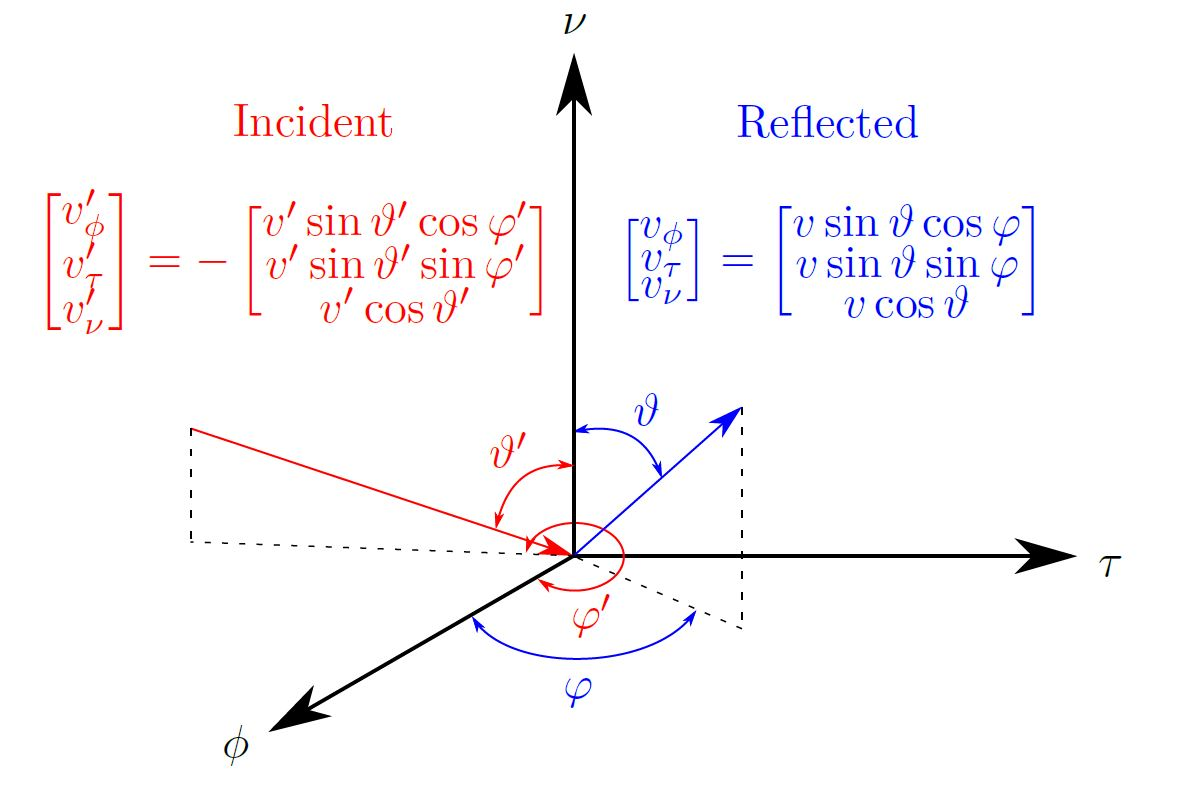
\includegraphics[width = 0.6\textwidth]{Figures/spherical_system.JPG}
	\caption{Transformation from the spherical $(v,\vartheta,\varphi)$ coordinate system to the Cartesian $(\phi,\tau,\nu)$ axis system.}
	\label{fig:spherical}
\end{figure}

We transform the velocity-dependent particle flux densities $\Gamma_{\nu-}^{a}(\xb,\vel')$ and $\Gamma_{\nu+}^{a}(\xb,\vel)$ to their speed- and angle-dependent equivalents $\Gamma_{\nu-}^{a}(\xb,v',\vartheta',\varphi')$ and $\Gamma_{\nu+}^{a}(\xb,v,\vartheta,\varphi)$. $\Gamma_{\nu-}^{a}(\xb,v',\vartheta',\varphi') \dd v' \dd \vartheta' \dd \varphi'$ and $\Gamma_{\nu+}^{a}(\xb,v,\vartheta,\varphi) \dd v \dd \vartheta \dd \varphi$ can be considered as respectively the incident and reflected particle flux densities of species $a$ at position $\xb$ for particles with a speed between $v^{(')}$ and $v^{(')} + \dd v^{(')}$, polar angle between $\vartheta^{(')} $ and $\vartheta^{(')} + \dd \vartheta^{(')}$ and azimuthal angle between $\varphi^{(')}$ and $\varphi^{(')} + \dd \varphi^{(')}$. The parentheses in the superscripts indicate that the prime is optional and only for the incident contribution. The speed- and angle-dependent particle flux density follows from the relation
\begin{align}
\Gamma_{\nu\pm}^{a}\left (\xb,v^{(')},\vartheta^{(')},\varphi^{(')} \right ) \dd v^{(')} \dd \vartheta^{(')} \dd \varphi^{(')} =& \ \Gamma_{\nu\pm}^{a} \left (\xb,\vel^{(')} \right ) \dd \vel^{(')} \nonumber \\
=& \ \Gamma_{\nu\pm}^{a}\left (\xb,\vel^{(')} \right ) \left (v^{(')}\right )^{2} \sin \vartheta^{(')} \dd v^{(')} \dd \vartheta^{(')} \dd \varphi^{(')}. \label{eq:spherical}
\end{align}

Splitting Eq.~\eqref{eq:kineticbc} explicitly into its fast and thermal contributions and using the speed- and angle-dependent distributions, gives

\begin{multline}
\Gammanplus(\xb,v,\vartheta,\varphi) = \int_{v'=0}^{\infty} \int_{\vartheta' = 0}^{\pi/2} \int_{\varphi' = 0}^{2\pi} R_{\mathrm{F}}(\xb;v',\vartheta',\varphi' \rightarrow v,\vartheta,\varphi) \sin \vartheta \ldots \\
\ldots \left( \Ri(\xb) \Gammaimin(\xb,v',\vartheta',\varphi') + \Rnx(\xb) \Gammanmin(\xb,v',\vartheta',\varphi') \right) \dd v' \dd \vartheta' \dd \varphi' \\
+ \frac{1}{\pi} \delta(v-\vT) \cos \vartheta \sin \vartheta \Gammanb{T}(\xb), \quad \text{for} \quad \xb \in \partial D, \label{eq:kineticbc2}
\end{multline}

\noindent with $R_{\mathrm{F}}(\xb;v',\vartheta',\varphi' \rightarrow v, \vartheta, \varphi)$ the fast reflection kernel from the TRIM database, $\delta(v)$ the Dirac delta function, $\vT$ the speed corresponding to the 2-3~eV Franck-Condon energy ($\efc$) and $\Gammanb{T}(\xb)$ the thermal particle flux density, given by
\begin{multline}
\Gammanb{T}(\xb) = \int_{v=0}^{\infty} \int_{\vartheta = 0}^{\pi/2} \int_{\varphi = 0}^{2\pi} \int_{v'=0}^{\infty} \int_{\vartheta' = 0}^{\pi/2} \int_{\varphi' = 0}^{2\pi} (1 - R_{\mathrm{F}}(\xb;v',\vartheta',\varphi' \rightarrow v, \vartheta,\varphi)) \ldots\\
\ldots \sin \vartheta (\Ri(\xb) \Gammaimin(\xb,v',\vartheta',\varphi') + \Rnx(\xb) \Gammanmin(\xb,v',\vartheta',\varphi')) \dd v \dd \theta \dd \phi \dd v' \dd \vartheta' \dd \varphi'. \label{eq:Gammant}
\end{multline}

In Section~\ref{sec:fion}, we determine $\Gammaimin(\xb,v',\vartheta',\varphi')$, which is the distribution of the incident ions. This distribution follows from the plasma solution. Then, we discuss how the fast reflection kernel $R_{\mathrm{F}}(\xb;v',\vartheta',\varphi' \rightarrow v,\vartheta,\varphi)$ is tabulated in the TRIM database in Section~\ref{sec:TRIM}. Finally, we explain in Section~\ref{sec:MCbc} how these boundary conditions are incorporated in the Monte Carlo procedure.

% ----------------------------------------------------------------------
\subsection{Velocity distribution of the incident ions}\label{sec:fion}
% ----------------------------------------------------------------------

Before proceeding to the elaboration of the velocity distribution, we briefly introduce the reader to the sheath boundary physics. At a solid boundary, there is a plasma-wall transition layer. If the magnetic field is oblique to the boundary surface, but with an angle between the magnetic field and surface tangential larger than approximately 5$^{\circ}$, the sheath region can be roughly subdivided in the quasi-neutral magnetic pre-sheath (Chodura sheath), with a width of the order of the ion gyroradius, and the electrostatic sheath (Debye sheath), with a width of the order of the Debye length $\lambda_{\mathrm{D}}$~\cite{chodura1982plasma,stangeby2012chodura}. The Debye length is given by

\begin{equation}
\lambda_{\mathrm{D}} = \left (\frac{\epsilon_{0} \Te}{\nne e^{2}} \right )^{1/2},
\end{equation}

with $\epsilon_{0}$ the permittivity of vacuum and $e$ the elementary charge. At the magnetic pre-sheath entrance, the Chodura condition states that the ion velocity parallel to the magnetic field reaches at least the isothermal speed of sound $\cs = \sqrt{(\Ti + \Te)/m}$. The electric field in the magnetic pre-sheath further accelerates the ions such that also the normal velocity reaches the isothermal speed of sound at the interface between the Chodura and Debye sheath, which is called the Bohm criterion. An extension of the description of the sheath layer for very small angles between the magnetic field and surface tangent (smaller than 5$^{\circ}$) can be found in Refs.~\cite{stangeby2012chodura, tskhakaya2005theory, tskhakaya2014comprehensive}.

The plasma fluid equations are not valid in the sheath region (Chodura and Debye sheaths). Therefore, one typically solves the plasma fluid equations up to the sheath entrance. However, for the neutral simulation, we need an expression for the ion distribution at the boundary surface to evaluate Eqs.~\eqref{eq:kineticbc}, \eqref{eq:kineticbc2}-\eqref{eq:Gammant}. In recent years, there were many efforts in the field of modeling the sheath region~\cite{cohen2004sheath, coulette2016kinetic, tskhakaya2014comprehensive}. However, we use a simplified model that neglects the deflection in the magnetic pre-sheath, similar as in the EIRENE code. It should be noted that the boundary conditions described below can be easily extended to a more elaborated sheath model, once this is implemented and tested in EIRENE.

From now on, we omit the explicit spatial dependence on $\xb$ in the notation. At the sheath entrance, the ion distribution is assumed to be a truncated Maxwellian, leading to

\begin{equation}
\Gamma_{\nu-,\mathrm{se}}^{\mathrm{i}}(\vel_{\mathrm{se}}) = \begin{cases} - C^{\mathrm{i}} \widetilde{M}(\vel_{\mathrm{se}};\Vi,\Ti) (\vel \cdot \Nu) & \text{if} \quad \vel_{\mathrm{se}} \cdot \Nu \leq 0, \\
0 & \text{otherwise}. \end{cases} \label{eq:truncMaxw}
\end{equation}

The constant scaling value $C^{\mathrm{i}}$ follows from the incident ion flux density:
\begin{equation}
\int_{\vel_{\mathrm{se}}} \Gamma_{\nu-,\mathrm{se}}^{\mathrm{i}}(\vel_{\mathrm{se}}) \dd \vel = - \nni (\Vi \cdot \Nu),
\end{equation}
in order to be consistent with the ion continuity equation. In the sheath region, the ions are accelerated perpendicular to the surface by the sheath potential difference $\Delta \phi_{\mathrm{sh}}$. We use the following simplified model for the sheath potential difference~\cite{stangeby1984plasma}:
\begin{equation}\label{eq:shpot}
\Delta \phi_{\mathrm{sh}} = \frac{\dshpot \Te}{e},
\end{equation}
with $\dshpot$ the sheath coefficient. If we express the particle velocity in the $(\phi,\tau,\nu)$ coordinate system of Fig.~\ref{fig:spherical}, then the velocity-dependent particle flux densities at the sheath entrance and boundary are related via
\begin{equation}
\Gamma_{\nu-,\mathrm{se}}^{\mathrm{i}}(v_{\phi,\mathrm{se}},v_{\tau,\mathrm{se}},v_{\nu,\mathrm{se}}) \dd v_{\phi,\mathrm{se}} \dd v_{\tau,\mathrm{se}} \dd v_{\nu,\mathrm{se}} = \Gammaimin(v_{\phi}',v_{\tau}',v_{\nu}') \dd v_{\phi}' \dd v_{\tau}' \dd v_{\nu}'. \label{eq:relationsheath}
\end{equation}
The tangential particle velocity components remain unchanged, i.e., $v_{\phi}' = v_{\phi,\mathrm{se}}$ and $v_{\tau}' = v_{\tau,\mathrm{se}}$, whereas the particle is accelerated by the sheath potential perpendicular to the surface, such that $\frac{m}{2}\left (v_{\nu}'\right )^{2} = \frac{m}{2} v_{\nu,\mathrm{se}}^{2} + \dshpot \Te$. Elaborating Eq.~\eqref{eq:relationsheath}, gives
\begin{equation}
\Gammaimin(v_{\phi}',v_{\tau}',v_{\nu}') = \begin{cases} -C^{\mathrm{i}} \widetilde{M} \Big (v_{\phi}',v_{\tau}',\ldots \\
 \quad \ldots -\sqrt{\left (v_{\nu}'\right )^{2} - \frac{2}{m} \dshpot\Te}; \Vi,\Ti \Big ) v_{\nu}' &  \text{if} \enskip v_{\nu}' \leq -v_{\mathrm{min}}, \\
0 & \text{otherwise}, \end{cases}
\end{equation}
with $v_{\mathrm{min}} = \sqrt{\frac{2}{m}\dshpot \Te}$ the minimum occurring velocity component perpendicular to the boundary after the sheath acceleration, and $\widetilde{M}(v_{\phi},v_{\tau},v_{\nu};{\bf V},T) = \widetilde{M}(\vel;{\bf V},T)$.

This velocity-dependent flux density can be used to evaluate Eq.~\eqref{eq:kineticbc}. However, the TRIM database is given in spherical coordinates (see Section~\ref{sec:TRIM}). Hence, we need an expression of the ion speed- and angle-dependent particle flux density to evaluate Eqs.~\eqref{eq:kineticbc2}-\eqref{eq:Gammant}. Using relation~\eqref{eq:spherical}, gives
\begin{equation}
\Gammaimin(v',\vartheta',\varphi') = \begin{cases} C^{\mathrm{i}} \finorm(v',\vartheta',\varphi';\dshpot) v' \sin \vartheta' \cos \vartheta' & \text{if} \quad v' \geq v_{\mathrm{min}}, \\
& \hspace{0.6cm} \vartheta' \leq \vartheta_{\mathrm{max}}, \\
0 & \text{otherwise}, \end{cases} \label{eq:fib}
\end{equation}
with $\vartheta_{\mathrm{max}} = \arccos (v_{\mathrm{min}}/v')$ and
\begin{multline}
\finorm(v',\vartheta',\varphi';\dshpot) = \left (v' \right )^{2} \widetilde{M} \Bigg (-v' \sin \vartheta' \cos \varphi',-v' \sin \vartheta' \sin \varphi', \ldots \\
\ldots -\sqrt{\left (v'\right )^{2} \cos^{2} \vartheta' -\frac{2}{m} \dshpot \Te};\Vi,\Ti \Bigg ). \label{eq:finormdshpot}
\end{multline}

Now, we have an expression for the speed- and angle-dependent particle flux density for the ions that can be plugged into Eqs.~\eqref{eq:kineticbc2}-\eqref{eq:Gammant}.

% ---------------------------------------------------------------------
\subsection{Reflection kernel from the TRIM database} \label{sec:TRIM}
% ---------------------------------------------------------------------

In this section, we explain how to extract the reflection kernel $R_{\mathrm{F}}(v',\vartheta',\varphi' \rightarrow v,\vartheta,\varphi)$ from the TRIM data tables. We omit the spatial dependence. Moreover, the reflection kernel becomes only spatially dependent if the vessel consists of different materials.

An expression for $R_{\mathrm{F}}(v',\vartheta',\varphi' \rightarrow v,\vartheta,\varphi)$ cannot be directly constructed from the database, because the tables are given as a function of the incident energy and polar angle. Hence, we first find an expression for $R_{\mathrm{F}}(E',\vartheta' \rightarrow E,\cos \vartheta,\cos \delta \varphi)$, with $E' \in [0,\infty]$, $\vartheta' \in [0,\pi/2]$ respectively the kinetic energy and angle with respect to the surface normal of the incident particle, and $E \in [0,E']$, $\vartheta \in [0,\pi/2]$ and $\delta \varphi \in [0, \pi]$ respectively the energy, angle with respect to the surface normal, and azimuthal angle deviation of the reflected/recycled particle. If $\delta \varphi = 0$, the tangential velocity of the recycled/reflected particle is in the same direction as the incident particle, whereas it is in the opposite direction for $\delta \varphi = \pi$.

The TRIM database consists of a total of 84 tables for different combinations of incident energies $E' = 1, 2, 5, 10, 20, 50, 100, 200, 500, 1\,000, 2\,000, \mathrm{and} 5\,000~eV$, and angles $\vartheta' = 0, 30, 45, 60, 70, 80, \mathrm{and} 85$ degrees. Every table contains the value for the particle reflection coefficient $R_{\mathrm{N}}(E',\vartheta')$, defined as
\begin{equation}
R_{\mathrm{N}}(E',\vartheta') = \int_{E = 0}^{E'} \int_{\cos \vartheta = 0}^{1} \int_{\cos \delta \varphi = -1}^{1} R_{\mathrm{F}}(E',\vartheta' \rightarrow E,\cos \vartheta,\cos \delta \varphi) \dd E \dd (\cos \vartheta) \dd (\cos \delta \varphi), \label{eq:RN}
\end{equation}
which is the probability that a particle with energy $E'$ and angle $\vartheta'$ is reflected as a fast atom.

The particle reflection coefficient $R_{\mathrm{N}}(E',\vartheta')$ only gives the probability of fast reflection, but for the distribution regarding the energy and direction of the recycled/reflected particle, we need extra information. For a certain combination of incident particle energy $E'$ and polar angle $\vartheta'$, three conditional distributions are tabulated: i) $R_{\mathrm{F}}(E',\vartheta' \rightarrow E)$ for the reflected energy distribution ($E$); ii) $R_{\mathrm{F}}(E',\vartheta' \rightarrow \cos \vartheta | E)$ for the polar angle distribution ($\cos \vartheta$) knowing that the recycled/reflected particle has energy $E$; and iii) $R_{\mathrm{F}}(E',\vartheta' \rightarrow \cos \delta \varphi | E, \cos \vartheta )$ for the azimuthal angle distribution ($\cos \delta \varphi$) after we know the recycled/reflected energy $E$ and (cosine of) the polar angle $\cos \vartheta$. These conditional distributions follow from
\begin{equation}
R_{\mathrm{F}}(E',\vartheta' \rightarrow E) = \left( \int_{\cos \vartheta = 0}^{1} \int_{\cos \delta \varphi = -1}^{1} R_{\mathrm{F}}(E',\vartheta' \rightarrow E,\cos \vartheta,\cos \delta \varphi) \dd (\cos \vartheta) \dd (\cos \delta \varphi) \right) / R_{\mathrm{N}}(E',\vartheta'),
\end{equation}
% -----------------------------------------------------------------------------------------------
\begin{equation}
R_{\mathrm{F}}(E',\vartheta' \rightarrow \cos \vartheta | E) = \left( \int_{\cos \delta \varphi = -1}^{1} R_{\mathrm{F}}(E',\vartheta' \rightarrow E,\cos \vartheta,\cos \delta \varphi) \dd (\cos \delta \varphi) \right) / \left( R_{\mathrm{N}}(E',\vartheta') R_{\mathrm{F}}(E',\vartheta' \rightarrow E) \right),
\end{equation}
% -------------------------------------------------------------------------------------------------
\begin{align}
R_{\mathrm{F}}(E',\vartheta' \rightarrow \cos \delta \varphi | E, \cos \vartheta ) =& \ R_{\mathrm{F}}(E',\vartheta' \rightarrow E,\cos \vartheta, \cos \delta \varphi)/ \left( R_{\mathrm{N}}(E',\vartheta') \right. \ldots \nonumber \\
\ldots & \left. R_{\mathrm{F}}(E',\vartheta' \rightarrow E) R_{\mathrm{F}}(E',\vartheta' \rightarrow \cos \vartheta | E) \right).
\end{align}
Then, the total reflection kernel can be written as
\begin{align}
R_{\mathrm{F}}(E',\vartheta' \rightarrow E,\cos \vartheta,\cos \delta \varphi) =& R_{\mathrm{N}}(E',\vartheta') R_{\mathrm{F}}(E',\vartheta' \rightarrow E) \ldots \nonumber \\
\ldots & R_{\mathrm{F}}(E',\vartheta' \rightarrow \cos\vartheta | E) R_{\mathrm{F}}(E',\vartheta' \rightarrow \cos \delta \varphi | E, \cos\vartheta).
\end{align}

\noindent These conditional distributions can be considered as three one-dimensional probability density functions. In the TRIM database, these distributions are discretized by means of five quantiles. We generalize the distribution as $R_{\mathrm{F}}(E',\vartheta' \rightarrow x), x \in [x_{\mathrm{min}},x_{\mathrm{max}}]$, with $x = E$ for the conditional energy distribution, $x = \cos \vartheta$ for the polar angle distribution, and $x = \cos \delta \varphi$ for the azimuthal angle distribution. Then, the cumulative distribution $F_{\mathrm{F}}(E',\vartheta' \rightarrow x)$ is defined as
\begin{equation}
F_{\mathrm{F}}(E',\vartheta' \rightarrow x) = \int_{x_{\mathrm{min}}}^{x} R_{\mathrm{F}}(E',\vartheta' \rightarrow y) \dd y.
\end{equation}
This distribution is discretized with five quantiles:
\begin{equation}
F_{\mathrm{F}}(E',\vartheta' \rightarrow x_{i}) = q_{i}, \quad \text{for} \quad i = 1, \ldots 5,
\end{equation}
with $q_{i} = 0.1 + 0.2(i-1)$. This is illustrated in Fig.~\ref{fig:reflection} (a), where the blue line represents the real cumulative distribution. The linear interpolation between these quantiles leads to a piecewise constant approximation for the probability density functions, as can be seen in Fig.~\ref{fig:reflection} (b).
\begin{figure}[ht]
	\centering
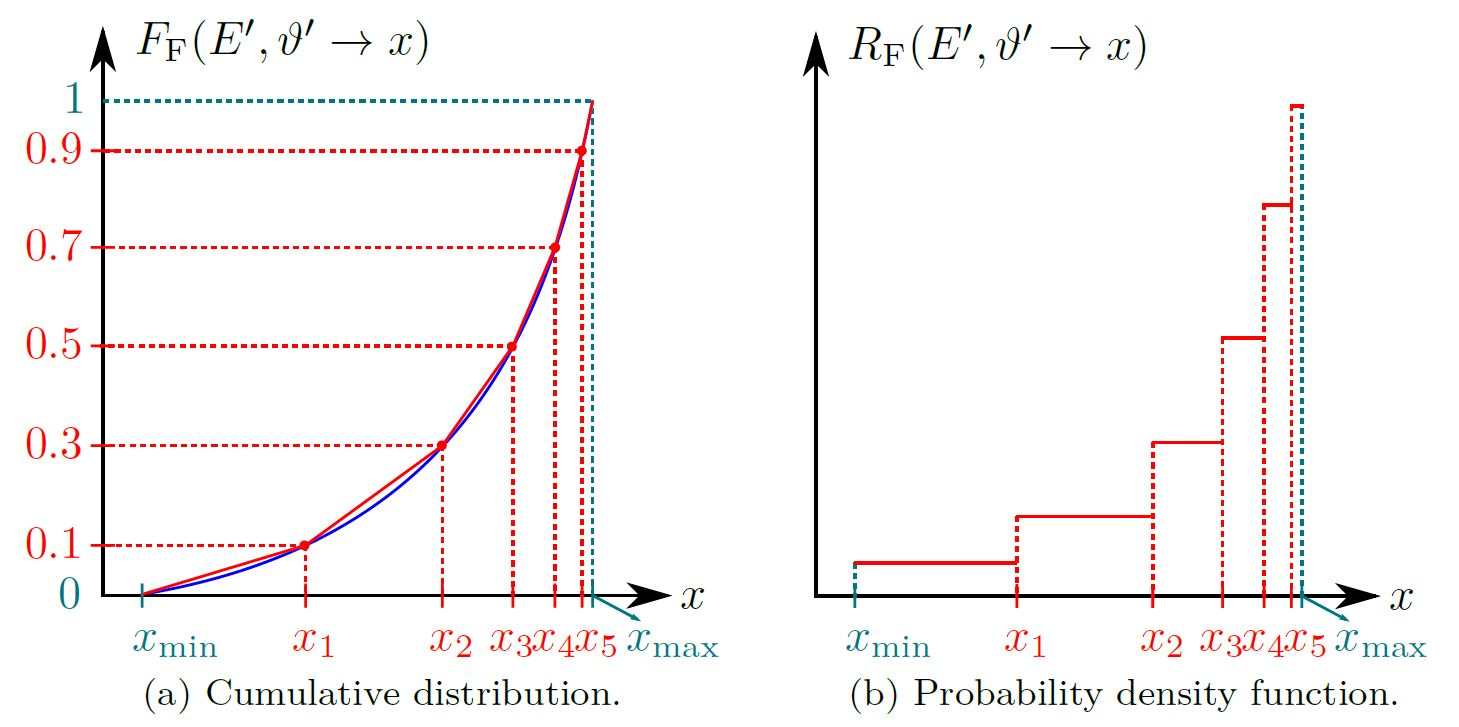
\includegraphics[width = 1.0\textwidth]{Figures/quantiles.JPG}
	\caption{Conditional cumulative distribution and probability density function from the TRIM database.}
 \label{fig:reflection}
\end{figure}

\noindent The cumulative distribution $F_{\mathrm{F}}(E',\vartheta' \rightarrow E)$ is discretized with five quantiles $E_{i}$ for every value of $E'$ and $\vartheta'$. Then for every quantile $E_{i}$, the function $F_{\mathrm{F}}(E',\vartheta' \rightarrow \cos \vartheta | E_{i})$ is discretized with five quantiles $\cos \vartheta_{j}$, thus, 25 additional numbers. Finally, the same is done for $F_{\mathrm{F}}(E',\vartheta' \rightarrow \cos \delta \varphi |E_{i}, \cos \vartheta_{j}$ (125 additional numbers). Hence, for every combination of $E'$ and $\vartheta'$ the TRIM database contains 155 numbers + 1 additional number for the reflection coefficient. Fig.~\ref{fig:trim} shows an example of a table from the TRIM database for a given incident energy-angle combination. The last number of the first line is the reflection coefficient $R_{\mathrm{N}}(E',\vartheta')$. The second line contains the quantiles for the reflected energy, the next five lines the quantiles for $\cos \vartheta$ for every value of $E$, and the next 25 lines contain the quantiles for $\cos \delta \varphi$ for every combination of $E$ and $\cos \vartheta$.

\begin{figure}[H]
	\centering
%	\def\svgwidth{160pt}
	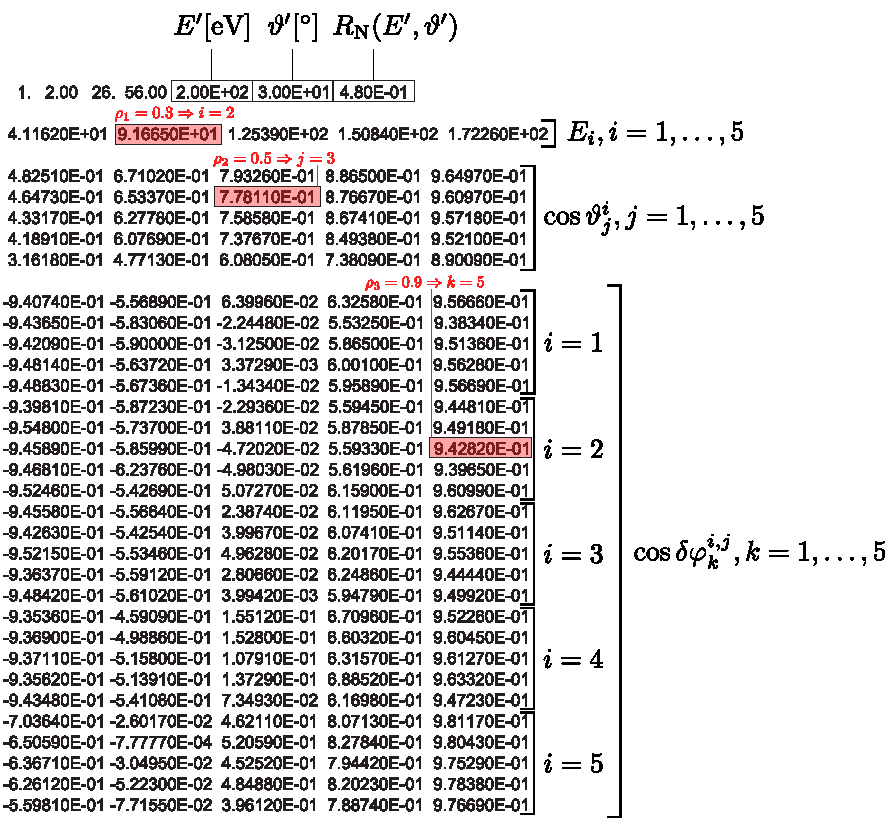
\includegraphics[width = 1.0\textwidth ]{Figures/trim.pdf}
	\caption[Data block from the TRIM database for $E' = 200$~eV and $\vartheta' = 30^{\circ}$.]{Data block from the TRIM database for $E' = 200$~eV and $\vartheta' = 30^{\circ}$~\cite{reiter2009eirene}.}
	\label{fig:trim}
\end{figure}

From the expression for $R_{\mathrm{F}}(E',\vartheta' \rightarrow E,\cos \vartheta, \cos \delta \varphi)$ we can derive the reflection kernel $R_{\mathrm{F}}(v',\vartheta',\varphi' \rightarrow v,\vartheta, \varphi)$ in Eq.~\eqref{eq:kineticbc2}, via the relation

\begin{equation}
R_{\mathrm{F}}(v',\vartheta',\varphi' \rightarrow v, \vartheta, \varphi) \sin \vartheta \dd v \dd \vartheta \dd \varphi = \frac{1}{2}R_{\mathrm{F}}(E',\vartheta' \rightarrow E, \cos \vartheta, \cos \delta \varphi) \dd E \left| \dd (\cos \vartheta) \dd (\cos \delta \varphi) \right| .
\end{equation}

In the right hand side, there appears a factor $1/2$, because of the equal probability that the particle is azimuthally deviating in the clockwise or counterclockwise directions compared to its original trajectory. With
\begin{equation}
E' = \frac{m}{2} (v')^{2}, \quad E = \frac{m}{2} v^{2}, \quad \varphi = \varphi' + \pi \pm \delta \varphi,
\end{equation}
this becomes
\begin{equation}
R_{\mathrm{F}}(v',\vartheta',\varphi' \rightarrow v, \vartheta, \varphi) = \frac{m}{2} v \left| \sin (\varphi - \varphi') \right| R_{\mathrm{F}} \left( \frac{m}{2} (v')^{2},\vartheta' \rightarrow \frac{m}{2} v^{2},\cos \vartheta, \cos (\varphi - \varphi') \right).
\end{equation}

% ---------------------------------------------------------------------
\subsection{Treatment of boundary conditions in Monte Carlo simulation} \label{sec:MCbc}
% ---------------------------------------------------------------------

\subsubsection{Application of the TRIM database}

The specific format for the TRIM tables facilitates the Monte Carlo simulation for the reflection of particles at a boundary. If a particle hits a boundary, its energy and incident polar angle are calculated. Then, the reflection coefficient $R_{\mathrm{N}}$ is determined by means of linear interpolation or extrapolation of the TRIM data. A random number $\rho$ from a uniform distribution between 0 and 1 is generated. If $\rho \leq R_{\mathrm{N}}$ the particle is reflected as a fast atom and the TRIM database is applied (option~1 below), otherwise the particle is thermally released (option~2 below).

\begin{itemize}
	\item \emph{Option~1: fast reflection.} Three uniformly distributed random numbers $\rho_{1}$, $\rho_{2}$ and $\rho_{3}$ (between 0 and 1) are generated. They determine respectively the reflected energy, polar angle and azimuthal angle. The reflected energy follows from
	\begin{equation}
	F_{\mathrm{F}}(E',\vartheta' \rightarrow E ) = \rho_{1},
	\end{equation}
	with the piecewise linear approximation of the cumulative distribution (Fig.~\ref{fig:reflection}(a)). Then, the polar angle is determined by
	\begin{equation}
	F_{\mathrm{F}}(E',\vartheta' \rightarrow \cos \vartheta | E) = \rho_{2},
	\end{equation}
	and finally, the relation for the azimuthal angle is
	\begin{equation}
	F_{\mathrm{F}}(E',\vartheta' \rightarrow \cos \delta \varphi | E,\cos \vartheta ) = \rho_{3}.
	\end{equation}
	
	For the three random numbers $\rho_{1} = 0.3$, $\rho_{2} = 0.5$ and $\rho_{3} = 0.9$ and an incident energy of 200~eV and polar angle of $30^{\circ}$ for the target-projectile combination of Fig.~\ref{fig:trim}, the resulting reflected energy and angles are indicated in the figure. For intermediate values of $E'$ and $\vartheta'$ and random numbers that do not exactly correspond with a tabulated quantile, linear interpolation/extrapolation of the tables is used.
	
	\item \emph{Option~2: thermal release.} In case of thermal release, the particle gets an energy of 2-3~eV. In order to have an isotropically distributed surface source (Lambert's cosine law), the polar angle has to be sampled from the probability density function $f(\vartheta)$, given by
	\begin{equation}
	f(\vartheta) = 2 \cos \vartheta \sin \vartheta, \quad \text{for} \quad \vartheta \in [0,\pi/2],
	\end{equation}
	as can be seen in Eq.~\eqref{eq:kineticbc2}~\cite{greenwood2002correct}. The corresponding cumulative distribution is
	\begin{eqnarray}
	F(\vartheta) &=& \int_{0}^{\vartheta} f(\vartheta') \dd \vartheta' \nonumber \\
	&=& \sin^{2} \vartheta.
	\end{eqnarray}
\noindent	Then, the polar angle follows from the relation
	\begin{equation}
	F(\vartheta) = \rho,
	\end{equation}
\noindent	with $\rho$ a random number uniformly distributed between 0 and 1. This leads to
	\begin{equation}
	\vartheta = \arcsin(\sqrt{\rho}).
	\end{equation}
\noindent	The azimuthal reflected angle is uniformly sampled between 0 and $2\pi$.
\end{itemize}

% ------------------------------------------------------
\section{Fluid boundary conditions} \label{sec:fluidbc}
% ------------------------------------------------------

In this section, we derive the boundary conditions for the fluid neutral models. The fluid models as described in literature use simple boundary conditions. E.g., a typical boundary condition for the parallel momentum equation is the momentum recycling boundary condition where the neutral parallel velocity at the target plate is assumed to be a constant fraction of the ion parallel velocity~\cite{rensink1998comparison,riemann2004navier}. However, this fraction is user-defined and not based on the underlying physics.

Here, we carefully derive the boundary conditions from the underlying kinetic physics. This is done by taking the particular moments of the neutral velocity distribution at the boundary. The total distribution consists of three parts: the incident neutrals, the reflected neutrals (an incident atom that is reflected as a fast or thermal atom) and the recycled neutrals (the incident ions that pick up an electron and are emitted as fast or thermal atoms). The distribution of the recycled neutrals can be calculated by taking the ion distribution at the boundary that entirely follows from the plasma macroscopic properties (Eq.~\eqref{eq:fib}), and multiplying it by the reflection kernel and integrating this product over the incident velocity space (Eqs.~\eqref{eq:kineticbc2}-\eqref{eq:Gammant}). The story is different for the reflected neutrals, because we need an expression for the distribution of the incident neutrals, but this can only be known by solving the kinetic equation. For the fluid models, we make an estimate for the distribution of these incident atoms.

The estimate is based on the diffusion approximation, as explained in Section~\ref{sec:diff}, or the drifting Maxwellian approximation, as explained in Section~\ref{sec:maxwellian}. Again, applying the reflection kernel leads to an estimate for the distribution of the reflected particles. In Section~\ref{sec:boundaryfluxes}, we take moments from the total distribution to obtain macroscopic fluxes. Finally, Section~\ref{sec:bcimplementation} deals with the practical implementation of these boundary conditions with imposed fluxes. It should be noted that the error introduced by the boundary conditions is fully due to the approximation for the incident neutrals. The TRIM reflection model is used for both the fluid and kinetic models and consequently, it does not introduce additional errors.


% ------------------------------------------------------
\subsection{Diffusion approximation for the distribution of the incident neutrals} \label{sec:diff}
% ------------------------------------------------------

Diffusion theory is frequently used in nuclear (fission) reactor physics~\cite{espinosa2011fractional, lamarsh1966introduction, park2012generation, piovezan2013heavy}. In our case, we will exclusively use it to estimate the distribution of the incident neutrals. We consider a control volume $\dd \mathcal{V}$ in which charge-exchange collisions scatter the neutrals in different directions, as indicated in Fig.~\ref{fig:diffusion}. We are interested in the number of neutrals that reach the area $\dd \mathcal{A}$ spanned by the solid angle $\dd \Omega$. $\dd \mathcal{A}$ is a surface element of the boundary (e.g., the target plate).
\begin{figure}[H]
	\centering
	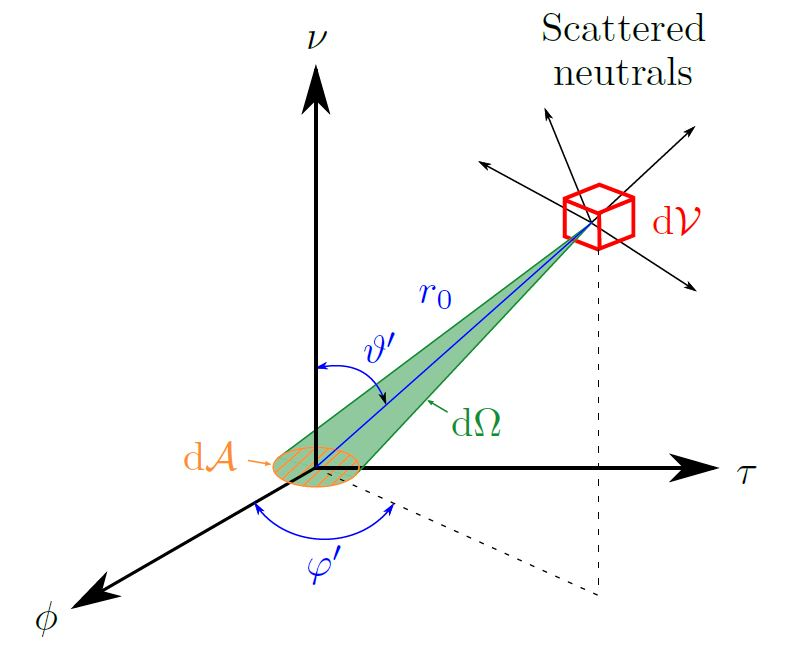
\includegraphics[width=0.5\textwidth]{Figures/scattering.JPG}
	\caption[Scattering of neutrals in control volume $\dd \mathcal{V}$.]{Scattering of neutrals in control volume $\dd \mathcal{V}$~\cite{nf_niels}.}
	\label{fig:diffusion}
\end{figure}

We calculate the speed- and angle-dependent particle flux density $\Gammanmin(v',\vartheta',\varphi')$ of neutrals scattered by the ions and reaching the plane $\dd \mathcal{A}$. We interpret $\Gammanmin(v',\vartheta',\varphi') \dd v' \dd \vartheta' \dd \varphi'$ as the number of neutrals per unit area per second reaching the surface element $\dd \mathcal{A}$ with a polar angle between $\vartheta'$ and $\vartheta' + \dd \vartheta'$, an azimuthal angle between $\varphi'$ and $\varphi' + \dd \varphi'$, and a speed between $v'$ and $v' + \dd v'$.

To calculate $\Gammanmin(v',\vartheta',\varphi')$, we need the source $S(v',\vartheta',\varphi')$ of neutrals created in the volume element $\dd \mathcal{V}$ with a speed between $v'$ and $v' + \dd v'$ scattered in the solid angle $\dd \Omega$. Charge-exchange collisions are assumed to be the main origin for neutral particles at a certain distance $r_{0}$. Thus, the source can be written as
\begin{equation}
S(v',\vartheta',\varphi') = \nn \nni \rcxm \finorm(v',\vartheta',\varphi'), \label{eq:S}
\end{equation}
which is the number of charge-exchange collisions per unit volume per second, multiplied with the normalized ion distribution $\finorm(v',\vartheta',\varphi')$. Here, $\nn$ is the neutral particle density, $\nni$ is the ion particle density, and $\rcxm$ is the momentum-linearized charge-exchange rate, as defined in Ref. \cite{nf_niels}.

The ion distribution in the domain is assumed to be a drifting Maxwellian $\left( \finorm(\vel') = \widetilde{M}(\vel';\Vi,\Ti) \right)$. This ion distribution is expressed as a function of the three velocity components and has to be transformed to the speed- and angle-dependent distribution as a function of $v'$, $\vartheta'$ and $\varphi'$. This is done with the transformation from Cartesian to spherical coordinates:
\begin{equation}
\finorm(\vel') \dd \vel' = \finorm(\vel') \left (v' \right )^{2} \dd v' \dd \Omega = \finorm(v',\vartheta',\varphi') \dd v' \dd \Omega.
\end{equation}
In this way, $\finorm(v',\vartheta',\varphi')$ becomes
\begin{align}
\finorm(v',\vartheta',\varphi') =& \left (v'\right )^{2} \widetilde{M}(\vel';\Vi,\Ti) \nonumber \\
=& \left (v'\right )^{2} \left( \frac{m}{2\pi\Ti} \right)^{3/2} \exp \left( -\frac{m}{2\Ti} \left( \left( v_{\phi}' - \ww \right)^{2} + \left(v_{\tau}' - u_{\tau} \right)^{2} + \left( v_{\nu}' - u_{\nu} \right)^{2} \right) \right).
\end{align}
Also transforming the Cartesian particle velocities to spherical coordinates, gives
\begin{multline}
\finorm(v',\vartheta',\varphi') = \left (v' \right)^{2} \left( \frac{m}{2\pi\Ti}\right)^{3/2} \times \\
\times \exp \left( -\frac{m}{2\Ti} \left( \left( v' \right)^{2} + 2 v' \sin \vartheta' \sin \varphi' u_{\tau} + 2 v' \sin \vartheta' \cos \varphi' u_{\phi} + 2 v' \cos \vartheta' u_{\nu} + u_{\phi}^{2} + u_{\tau}^{2} + u_{\nu}^{2} \right) \right). \label{eq:finorm}
\end{multline}

\noindent This source has to be multiplied with the probability that the neutral reaches the boundary plane without any extra collision (probability of non-absorption $P_{\mathrm{NA}}(v')$). This probability is given by
\begin{equation}
P_{\mathrm{NA}}(v') = \exp \left( -\St(v') r_{0} \right), \label{eq:PNA}
\end{equation}
with $\St(v') = (\nni\rcxm + \nne\rion)/v'$ the total macroscopic cross-section (including charge-exchange and ionization events).

Then, the speed- and angle-dependent particle flux density becomes
\begin{equation}
\Gammanmin(v',\vartheta',\varphi') \dd v' \dd \vartheta' \dd \varphi' \dd \mathcal{A} = \int_{\mathcal{V}} S(v',\vartheta',\varphi') P_{\mathrm{NA}}(v') \dd \mathcal{V} \dd v' \dd \Omega. \label{eq:Gammanmin1}
\end{equation}
To obtain the total particle flux density, the integral over the whole domain volume has to be taken. If the total macroscopic cross-section is large, the exponential term $e^{-\St(v') r_{0}}$ in $P_{\mathrm{NA}}(v')$ (Eq.~\eqref{eq:PNA}) decays rapidly. Therefore, only the first few mean free paths starting from the boundary contribute to the integral of Eq.~\eqref{eq:Gammanmin1}, and we can replace the integral over the edge plasma domain by a semi-infinite integral with $r_{0} \in [0,\infty )$. The solid angle spanned by $\dd \mathcal{A}$ is $\dd \mathcal{A} \frac{\cos\vartheta'}{r_{0}^{2}}$ and the volume $\dd \mathcal{V}$ is $r_{0}^{2}\sin \vartheta' \dd r_{0} \dd \vartheta' \dd \varphi'$. Inserting all expressions in Eq.~\eqref{eq:Gammanmin1}, gives
\begin{equation}
\Gammanmin(v',\vartheta',\varphi') = \int_{r_{0}=0}^{\infty} e^{-\St(v') r_{0}} \nn \nni \rcxm \finorm(v',\vartheta',\varphi') \sin \vartheta' \cos \vartheta' \dd r_{0}. \label{eq:Gammanmin2}
\end{equation}
We use a Taylor series expansion for the neutral density:
\begin{eqnarray}
\nn &\approx& n_{\mathrm{n}_{0}} + \phi \left (\ddx{\nn}{\phi}\right )_{0} + \tau \left (\ddx{\nn}{\tau}\right )_{0} + \nu \left (\ddx{\nn}{\nu} \right )_{0} \nonumber \\
&=& n_{\mathrm{n}_{0}} + r_{0} \sin \vartheta' \sin \varphi' \left (\ddx{\nn}{\tau}\right )_{0}  + r_{0} \cos \vartheta' \left (\ddx{\nn}{\nu} \right )_{0},
\end{eqnarray}
assuming toroidal symmetry such that $(\partial \nn/\partial \phi)_{0} = 0$. The subscript 0 indicates that the neutral density and gradients are evaluated in the origin, where the particle flux density is calculated. Inserting this expression for the neutral density in Eq.~\eqref{eq:Gammanmin2}, gives
\begin{align}
\Gammanmin(v',\vartheta',\varphi') = \int_{r_{0}=0}^{\infty} & e^{-\St(v') r_{0}} \left( \nn + r_{0} \sin \vartheta' \sin \varphi' \left( \ddx{\nn}{\tau} \right) + r_{0} \cos \vartheta' \left( \ddx{\nn}{\nu}\right) \right) \times \nonumber \\
\times & \nni \rcxm \finorm(v',\vartheta',\varphi') \sin \vartheta' \cos \vartheta' \dd r_{0}, \label{eq:Gammanmin3}
\end{align}
where the subscript $0$ is omitted for simplicity of notation. Finally, evaluating the integral neglecting the spatial dependence of $\St$, $\nni \rcxm$, and $\finorm$, gives
\begin{align}
\Gammanmin(v',\vartheta',\varphi') =& \frac{\nni \rcxm}{\nni \rcxm + \nne \rion} \finorm(v',\vartheta',\varphi') v' \sin \vartheta' \cos \vartheta' \times \nonumber \\
\times & \left( \nn + \frac{v'}{\nni\rcxm + \nne \rion} \left( \sin \vartheta' \sin \varphi' \ddx{\nn}{\tau} + \cos \vartheta' \ddx{\nn}{\nu} \right) \right) \label{eq:Gammanmin}
\end{align}

Due to the exponential decay term in Eq.~\eqref{eq:Gammanmin3}, only the first mean free paths away from the boundary contribute to the integral and the spatial variations of $\St$, $\nni\rcxm$, and $\finorm$ can be assumed to be small in this region. Basically, this means that the Knudsen number has to be sufficiently small, which is also a necessary condition for the use of a fluid model in the bulk of the domain. Indeed, a small Knudsen number means that the macroscopic length scales of the parameters in the integrand of Eq.~\eqref{eq:Gammanmin3} are large compared to the neutral mean free path length ($1/\St$). These large macroscopic length scales compared to the mean free path length lead to relatively small variations of the macroscopic properties in the exponentially decaying region that contributes to the integral.

% ------------------------------------------------------
\subsection{Truncated drifting Maxwellian approximation for the distribution of the incident neutrals} \label{sec:maxwellian}
% ------------------------------------------------------

The diffusion approximation for the incident neutrals was shown to be accurate for the target boundary conditions in \cite{nf_niels} and \cite{pet_maarten}. However, this boundary condition requires a short mean free path to be valid, and it was found that unphysical behavior can arise when the mean free path is too long. Therefore, an alternative model was developed, assuming a truncated drifting Maxwellian distribution for the incident neutrals, based on the macroscopic neutral density, velocity, and temperature at the target:

\begin{align}
\Gammanmin(v',\vartheta',\varphi') =&  \fnnorm(v',\vartheta',\varphi') v' \sin \vartheta' \cos \vartheta'. \label{eq:Gammanmin_maxw}
\end{align}

Here, the normalized neutral distribution is
\begin{align}
\fnnorm(v',\vartheta',\varphi') =& \left( v' \right)^{2} \widetilde{M} (\vel';\Vn,\Tn) \nonumber \\
=& \left( v' \right)^{2} \left( \frac{m}{2\pi\Tn} \right)^{3/2} \exp \left( -\frac{m}{2\Tn} \left( \left( v_{\phi}' - \wwn \right)^{2} + \left( v_{\tau}' - u_{\mathrm{n}\tau} \right)^{2} + \left( v_{\nu}' - u_{\mathrm{n}\nu} \right)^{2} \right) \right).
\end{align}

Again transforming the Cartesian particle velocities to spherical coordinates, gives
\begin{multline}
\fnnorm(v',\vartheta',\varphi') = \left (v'\right )^{2} \left (\frac{m}{2\pi\Tn}\right )^{3/2} \exp \bigg (-\frac{m}{2\Tn} \Big (\left (v'\right )^{2} + 2 v' \sin \vartheta' \sin \varphi' u_{\mathrm{n}\tau} + \\
+ 2 v' \sin \vartheta' \cos \varphi' u_{\mathrm{n}\phi}
+ 2 v' \cos \vartheta' u_{\mathrm{n}\nu} + u_{\mathrm{n}\phi}^{2} + u_{\mathrm{n}\tau}^{2} + u_{\mathrm{n}\nu}^{2} \Big ) \bigg ). \label{eq:fnnorm}
\end{multline}

This option was found to be slightly less accurate than the diffusion approximation for high collisional cases \cite{nf_wim}, but still far more accurate than previous {\it ad hoc} fluid neutral boundary conditions, while being more robust in the regions with larger neutral mean free paths.
From now on, we use the superscripts `diff' and `Maxw' to differentiate between the diffusion and Maxwellian options, when the distinction needs to be made explicit.

% ------------------------------------------------------
\subsection{Resulting macroscopic boundary fluxes} \label{sec:boundaryfluxes}
% ------------------------------------------------------

From the distributions of the incident neutrals and ions, the net fluxes at the boundaries can be calculated. In our case, the speed and angular distributions of the fast recycled and reflected neutrals are determined by the TRIM code database, whereas the thermally released neutrals are emitted diffusely with an energy of 2-3~eV. Below, we elaborate the particle, parallel momentum, and energy flux density.

% ------------------------------------------------------
\subsubsection{Neutral particle flux density}

\noindent The net neutral particle flux density $\Gamma^{\mathrm{n}} = \nn \Vn \cdot \Nu$ constitutes of four contributions:
\begin{equation}
\Gamma^{\mathrm{n}} =  \Gamma_{\mathrm{refl},\mathrm{f}}^{\mathrm{n}} + \Gamma_{\mathrm{rec},\mathrm{f}}^{\mathrm{n}} + \Gammanb{T} - \Gamma_{\nu-}^{\mathrm{n}},
\end{equation}
with $\Gamma_{\mathrm{refl},\mathrm{f}}^{\mathrm{n}}$ and $\Gamma_{\mathrm{rec},\mathrm{f}}^{\mathrm{n}}$ respectively the fast reflected and recycled particle flux density (as described by the TRIM database) and $\Gammanb{T}$ the thermally released fraction, decreased with the incident particle flux density $\Gamma_{\nu-}^{\mathrm{n}}$. These contributions are elaborated with the help of the particle reflection coefficient (Eq.~\eqref{eq:RN}):
\begin{align}
\Gamma_{\nu-}^{\mathrm{n}} =& \int_{v'=0}^{\infty} \int_{\vartheta'=0}^{\pi/2} \int_{\varphi'=0}^{2\pi} \Gamma_{\nu-}^{\mathrm{n}}(v',\vartheta',\varphi') \dd v' \dd \vartheta' \dd \varphi', \label{eq:Gammanin} \\
\Gamma_{\mathrm{refl},\mathrm{F}}^{\mathrm{n}} =& \ \Rnx \int_{v'=0}^{\infty} \int_{\vartheta'=0}^{\pi/2} \int_{\varphi'=0}^{2\pi} R_{\mathrm{N}}(v',\vartheta') \Gamma_{\nu-}^{\mathrm{n}}(v',\vartheta',\varphi') \dd v' \dd \vartheta' \dd \varphi', \label{eq:Gammarefl} \\
\Gamma_{\mathrm{rec},\mathrm{F}}^{\mathrm{n}} =& \ \Ri \int_{v'=0}^{\infty} \int_{\vartheta'=0}^{\pi/2} \int_{\varphi'=0}^{2\pi} R_{\mathrm{N}}(v',\vartheta') \Gamma_{\nu-}^{\mathrm{i}}(v',\vartheta',\varphi') \dd v' \dd \vartheta' \dd \varphi', \label{eq:Gammarec}
\end{align}
\begin{align}
\Gammanb{T} = \int_{v'=0}^{\infty} \int_{\vartheta'=0}^{\pi/2} \int_{\varphi'=0}^{2\pi} \left( 1 - R_{\mathrm{N}}(v',\vartheta') \right) \left( \Rnx \Gammanmin(v',\vartheta',\varphi') + \Ri \Gammaimin(v',\vartheta',\varphi') \right) \dd v' \dd \vartheta' \dd \varphi'. \label{eq:GammanT}
\end{align}

It should be noted that the particle reflection coefficient is written as a function of the incident speed $v'$ and not as function of the incident energy $E' = \frac{m}{2}(v')^{2}$ in Eq.~\eqref{eq:RN}.

% -------------------------------------------------------
\subsubsection{Neutral parallel momentum flux density}


Similar to the net neutral particle flux density, the neutral parallel momentum flux density $\Gamma_{\mathrm{m},||}^{\mathrm{n}}$ becomes

\begin{align}
\Gamma_{\mathrm{m},||}^{\mathrm{n}} =& \left[ \left( m\nn\Vn\Vn + \viscn + \pn \mathds{I} \right) \cdot \Nu \right]_{||} \label{eq:momfluxp} \\
=& \ m \int_{v'=0}^{\infty} \int_{\vartheta'=0}^{\pi/2} \int_{\varphi'=0}^{2\pi} \Bigg [ \underbrace{-v'_{||} \Gamma_{\nu-}^{\mathrm{n}}(v',\vartheta',\varphi')}_{\text{incident}} \nonumber \\
& + \underbrace{\int_{v=0}^{v'} \int_{\vartheta=0}^{\pi/2} \int_{\varphi=0}^{2\pi} v_{||}  R_{\mathrm{F}}(v',\vartheta',\varphi' \rightarrow v, \vartheta,\varphi)\sin \vartheta \dd v \dd \vartheta \dd \varphi\ldots}_{\text{fast}} \nonumber \\
&\qquad \underbrace{\ldots \left (\Rnx \Gamma_{\nu-}^{\mathrm{n}}(v',\vartheta',\varphi') + \Ri \Gamma_{\nu-}^{\mathrm{i}}(v',\vartheta',\varphi')\right )}_{\text{fast}} \Bigg ] \dd v' \dd \vartheta' \dd \varphi' + \underbrace{\Gamma_{\mathrm{m},||,\mathrm{T}}^{\mathrm{n}}}_{\text{thermal}}, \label{eq:Gammamp}
\end{align}

\noindent with $v_{||} = \pit (\sin \alpha_{\nu} v_{\tau} + \cos \alpha_{\nu} v_{\nu}) + \pitt v_{\phi}$ the neutral particle velocity parallel to the magnetic field, and $\alpha_{\nu}$ the angle between the surface normal and the poloidal direction. The different contributions are indicated with sub braces. To write Eq.~\eqref{eq:Gammamp} more compactly, we make use of the parallel and perpendicular momentum reflection coefficients, respectively $R_{\mathrm{m},||}(v',\vartheta')$ and $R_{\mathrm{m},\perp}(v',\vartheta')$. Then, Eq.~\eqref{eq:Gammamp} becomes
\begin{align}
\Gamma_{\mathrm{m},||}^{\mathrm{n}} =& \ m \int_{v'=0}^{\infty} \int_{\vartheta'=0}^{\pi/2} \int_{\varphi'=0}^{2\pi} \Bigg[ \underbrace{- v'_{||} \Gamma_{\nu-}^{\mathrm{n}}(v',\vartheta',\varphi')}_{\text{incident}} +  \underbrace{\bigg (- \pitt R_{\mathrm{m},||}(v',\vartheta') \ldots}_{\text{fast}}  \nonumber \\
& \underbrace{\ldots  \sin \vartheta' \cos \varphi' - \pit \sin \alpha_{\nu} R_{\mathrm{m},||}(v',\vartheta') \sin \vartheta' \sin \varphi' + \pit \cos \alpha_{\nu}  \ldots}_{\text{fast}} \nonumber \\
&\underbrace{\ldots R_{\mathrm{m},\perp}(v',\vartheta') \cos \vartheta' \bigg ) v' \left( \Rnx \Gamma_{\nu-}^{\mathrm{n}}(v',\vartheta',\varphi') + \Ri \Gamma_{\nu-}^{\mathrm{i}}(v',\vartheta',\varphi') \right)}_{\text{fast}} \Bigg] \dd v' \dd \vartheta' \dd \varphi' + \ldots \nonumber \\
&\ldots + \underbrace{\Gamma_{\mathrm{m},||,\mathrm{T}}^{\mathrm{n}}}_{\text{thermal}}, \label{eq:Gammanmomp}
\end{align}
with
\begin{align}
R_{\mathrm{m},||}(v',\vartheta') = \frac{1}{mv'\sin\vartheta'} \int_{v=0}^{v'} \int_{\vartheta=0}^{\pi/2}\int_{\varphi=0}^{2\pi} m v \sin\vartheta \cos \varphi R_{\mathrm{F}}(v',\vartheta',0 \rightarrow v,\vartheta,\varphi) \sin \vartheta \dd v \dd \vartheta \dd \varphi, \label{eq:Rmpar}
\end{align}
\begin{align}
R_{\mathrm{m},\perp}(v',\vartheta') = \frac{1}{mv'\cos \vartheta'} \int_{v=0}^{v'} \int_{\vartheta=0}^{\pi/2} \int_{\varphi=0}^{2\pi} m v \cos \vartheta R_{\mathrm{F}}(v',\vartheta',0 \rightarrow v,\vartheta,\varphi) \sin \vartheta \dd v \dd \vartheta \dd \varphi. \label{eq:Rmperp}
\end{align}

The parallel momentum reflection coefficient represents the mean fraction of momentum that is conserved in the direction of motion of the incident particle projected on the boundary plane multiplied by the probability of fast reflection $R_{\mathrm{N}}(v',\vartheta')$. The perpendicular momentum reflection coefficient represents the ratio of the momentum perpendicular to the plane of the reflected and incident particle again multiplied by $R_{\mathrm{N}}(v',\vartheta')$. The calculation of these reflection coefficients is treated in Section~\ref{sec:bcimplementation}.

The thermally released neutrals are emitted isotropically (Lambert's cosine law), leading to the following parallel momentum flux density:
\begin{align}\label{eq:par_momentum_T}
\Gamma_{\mathrm{m},||,\mathrm{T}}^{\mathrm{n}} =& \ m \int_{v=0}^{\infty} \int_{\vartheta = 0}^{\pi/2} \int_{\varphi = 0}^{2\pi} v_{||} \frac{1}{\pi} \delta(v - \vT) \cos \vartheta \sin \vartheta \Gammanb{T} \nonumber \\
=& \ \pit \cos \alpha_{\nu} \frac{2}{3} m \vT \Gammanb{T}.
\end{align}

As can be seen in Eq.~\eqref{eq:momfluxp}, this parallel momentum flux density includes the pressure. However, for fluid models, it is typical to consider the pressure gradient as a driving force rather than a flux contribution. The parallel momentum flux density from the fluid point of view (subscript $\mathrm{f}$) becomes
\begin{equation}
\Gamma_{\mathrm{m},\mathrm{f},||}^{\mathrm{n}} = \left [\Gamma_{\mathrm{m,f}}^{\mathrm{n}} \cdot \Nu\right ]_{||} = \Gamma_{\mathrm{m},||}^{\mathrm{n}} - \pit \cos \alpha_{\nu} \pn, \label{eq:Gammamompf}
\end{equation}
i.e., excluding the pressure contribution.

There are two possible choices for the pressure at a certain position at a boundary. One can take the pressure that follows from the fluid solution. However, at the boundaries, the underlying velocity distribution deviates a lot from the Maxwellian equilibrium distribution. Therefore, it is recommended to recalculate the pressure from the estimated distribution that consists of the incident, recycled, and reflected neutrals. If the total velocity-dependent particle flux density at a boundary is $\Gamma^{\mathrm{n}}(\vel)$, the pressure is defined as
\begin{equation}
\pn' = \frac{m}{3} \int ||\vel -\Vn'||^{2} \frac{\Gamma^{\mathrm{n}}(\vel)}{|v_{\nu}|} \dd \vel, \label{eq:pnboundary}
\end{equation}
where the prime is used to indicate that the macroscopic quantity is recalculated from the estimated underlying velocity distribution $\Gamma^{\mathrm{n}}(\vel)/|v_{\nu}|$ at the boundary, and consequently, it might differ from the quantity that results from the fluid solution. This is not only the case for the pressure, but also for the density ($\nn' = \int \frac{\Gamma^{\mathrm{n}}(\vel)}{|v_{\nu}|} \dd \vel$) and velocity ($\Vn' = \frac{1}{\nn'}\int \vel \frac{\Gamma^{\mathrm{n}}(\vel)}{|v_{\nu}|} \dd \vel$).

Elaborating Eq.~\eqref{eq:pnboundary}, gives
\begin{equation}
\pn' = \underbrace{\frac{m}{3} \int ||\vel||^{2} \frac{\Gamma^{\mathrm{n}}(\vel)}{|v_{\nu}|} \dd \vel}_{(1)} - \underbrace{\frac{m}{3} \nn' || \Vn'||^{2}}_{(2)}. \label{eq:pnboundary2}
\end{equation}
Term~(1) is the total second order moment with a contribution from the fluid velocity $\Vn'$ that has to be subtracted to obtain the pressure (term~(2)).

Elaborating term~(1) of Eq.~\eqref{eq:pnboundary2}, gives
\begin{multline}
\frac{m}{3} \int ||\vel||^{2} \frac{\Gamma^{\mathrm{n}}(\vel)}{|v_{\nu}|} \dd \vel = \frac{m}{3} \int_{v'=0}^{\infty} \int_{\vartheta'=0}^{\pi/2} \int_{\varphi'=0}^{2\pi} \left [ \underbrace{\left (v'\right )^{2} \frac{\Gamma_{\nu-}^{\mathrm{n}}(v',\vartheta',\varphi')}{v' \cos \vartheta'}}_{\text{incident}} \right.  \\
\left. + \underbrace{R_{p}(v',\vartheta') \left (v' \right )^{2}  \frac{\Rnx \Gamma_{\nu-}^{\mathrm{n}}(v',\vartheta',\varphi') + \Ri \Gamma_{\nu-}^{\mathrm{i}}(v',\vartheta',\varphi')}{v' \cos \vartheta'}}_{\text{fast}} \right ] \dd v' \dd \vartheta' \dd \varphi' + \underbrace{\frac{2}{3} m \vT \Gammanb{T}}_{\text{thermal}}, \label{eq:v2fn}
\end{multline}
with
\begin{align}
R_{p}(v',\vartheta') = \frac{\cos \vartheta'}{v'} \int_{v=0}^{v'} \int_{\vartheta=0}^{\pi/2} \int_{\varphi=0}^{2\pi} \frac{v}{\cos \vartheta} R_{\mathrm{F}}(v',\vartheta',0 \rightarrow v,\vartheta,\varphi) \sin \vartheta \dd v \dd \vartheta \dd \varphi, \label{eq:Rp}
\end{align}
a reflection coefficient that determines the second order moment of the distribution after reflection.

Now, we elaborate term~(2) of Eq.~\eqref{eq:pnboundary2}. Therefore, we need an expression for the density $\nn'$ and the velocity $\Vn'$. To calculate these quantities, we need the distributions of the different contributions, i.e., the distribution of the incident, fast reflected/recycled, and thermally released neutrals, respectively $f_{\mathrm{n},\nu-}(v',\vartheta',\varphi')$, $f_{\mathrm{n},\nu+,\mathrm{f}}(v,\vartheta,\varphi)$, and $f_{\mathrm{n},\nu+,\mathrm{T}}(v,\vartheta,\varphi)$, given by
\begin{align}
f_{\mathrm{n},\nu-}(v',\vartheta',\varphi') =& \frac{\Gamma_{\nu-}^{\mathrm{n}}(v',\vartheta',\varphi')}{v'\cos \vartheta' \sin \vartheta'}, \\
f_{\mathrm{n},\nu+,\mathrm{f}}(v,\vartheta,\varphi) =& \int_{v'=0}^{\infty} \int_{\vartheta'=0}^{\pi/2} \int_{\varphi'=0}^{2\pi} R_{\mathrm{F}}(v',\vartheta',\varphi' \rightarrow v,\vartheta,\varphi) \sin \vartheta \ldots \nonumber \\
&\ldots \frac{\Rnx \Gamma_{\nu-}^{\mathrm{n}}(v',\vartheta',\varphi') + \Ri \Gamma_{\nu-}^{\mathrm{i}}(v',\vartheta',\varphi')}{v \cos \vartheta \sin \vartheta} \dd v' \dd \vartheta' \dd \varphi', \label{eq:fnplusf} \\
f_{\mathrm{n},\nu+,\mathrm{T}}(v,\vartheta,\varphi) =& \frac{\Gamma_{\mathrm{T}}^{\mathrm{n}}}{\pi \vT} \delta (v - \vT).
\end{align}
The zeroth order moment of the total distribution leads to an expression for $\nn'$:
\begin{align}
\nn' = \int_{v'=0}^{\infty} \int_{\vartheta'=0}^{\pi/2} \int_{\varphi'=0}^{2\pi} &
f_{\mathrm{n},\nu-}(v',\vartheta',\varphi') \sin \vartheta' \dd v' \dd \vartheta' \dd \varphi' \nonumber \\
+ \int_{v=0}^{\infty} \int_{\vartheta = 0}^{\pi/2} \int_{\varphi = 0}^{2\pi} & \left( f_{\mathrm{n},\nu+,\mathrm{f}}(v,\vartheta,\varphi) + f_{\mathrm{n},\nu+,\mathrm{T}}(v,\vartheta,\varphi) \right) \sin \vartheta \dd v \dd \vartheta \dd \varphi \nonumber \\
= \int_{v'=0}^{\infty} \int_{\vartheta' = 0}^{\pi/2} \int_{\varphi' = 0}^{2\pi} & \bigg[ \frac{\Gamma_{\nu-}^{\mathrm{n}}(v',\vartheta',\varphi')}{v' \cos \vartheta'} + \frac{R_{\nn}(v',\vartheta')}{v' \cos \vartheta'} \left( \Rnx \Gamma_{\nu-}^{\mathrm{n}}(v',\vartheta',\varphi') \right. \nonumber \\
& \left. + \Ri \Gamma_{\nu-}^{\mathrm{i}}(v',\vartheta',\varphi') \right) \bigg] \dd v' \dd \vartheta' \dd \varphi' + \frac{2}{\vT} \Gamma_{\mathrm{T}}^{\mathrm{n}}, \label{eq:nnboundary}
\end{align}
with the density reflection coefficient $R_{\nn}(v',\vartheta')$, defined as
\begin{align}
R_{n_{\mathrm{n}}}(v',\vartheta') = v' \cos \vartheta' \int_{v=0}^{v'} \int_{\vartheta=0}^{\pi/2} \int_{\varphi=0}^{2\pi} \frac{1}{v \cos \vartheta} R_{\mathrm{F}}(v',\vartheta',0 \rightarrow v,\vartheta,\varphi) \sin \vartheta \dd v \dd \vartheta \dd \varphi. \label{eq:Rnn}
\end{align}
This coefficient guarantees the particle balance of the recycled/reflected neutrals. If there is a strong reduction of the perpendicular velocity after reflection, the density has to increase to guarantee that the reflected/recycled particle flux density is the incident particle flux density multiplied by the probability of fast reflection.

Finally, we need an expression for $\Vn'$, the last missing factor to calculate the pressure with Eq.~\eqref{eq:pnboundary2}. Assuming that $\wwn' \gg u_{\mathrm{n}\tau}', u_{\mathrm{n}\nu}'$, gives
\begin{equation}
\frac{m}{3} \nn' ||\Vn'||^{2} \approx \frac{m}{3} \nn' \wwn'^{2}, \label{eq:pnboundary_term2}
\end{equation}
such that we only have to calculate the toroidal component $\wwn'$ from the underlying estimated distribution. This assumption is in accordance to the ones made for the parallel momentum equation \cite{nf_niels}, where it is assumed that the neutral parallel velocity is at least an order of magnitude larger than the radial and diamagnetic components. For small pitches, the toroidal and parallel components are almost the same. The toroidal velocity follows from
\begin{align}
\nn' \wwn' =& \int_{v'=0}^{\infty} \int_{\vartheta'=0}^{\pi/2} \int_{\varphi'=0}^{2\pi} \Bigg [\underbrace{-v' \sin \vartheta' \cos \varphi' \frac{\Gamma_{\nu-}^{\mathrm{n}}(v',\vartheta',\varphi')}{v' \cos \vartheta'}}_{\text{incident}}  \nonumber \\
&+ \underbrace{\int_{v=0}^{v'} \int_{\vartheta=0}^{\pi/2} \int_{\varphi=0}^{2\pi} v \sin \vartheta \cos \varphi R_{\mathrm{F}}(v',\vartheta',\varphi' \rightarrow v,\vartheta,\varphi) \sin \vartheta \dd v \dd \vartheta \dd \varphi  \ldots}_{\text{fast}} \nonumber \\
&\underbrace{ \ldots \frac{\Rnx \Gamma_{\nu-}^{\mathrm{n}}(v',\vartheta',\varphi') + \Ri \Gamma_{\nu-}^{\mathrm{i}}(v',\vartheta',\varphi')}{v' \cos \vartheta'} \Bigg ] \dd v' \dd \vartheta' \dd \varphi'}_{\text{fast}}. \label{eq:nnwwn}
\end{align}
There is no contribution from the thermal neutrals to $\wwn'$ due to the isotropic emission. Again, Eq.~\eqref{eq:nnwwn} can be simplified by defining a reflection coefficient for the inner integrals over $v$, $\vartheta$ and $\varphi$:
\begin{equation}
R_{\wwn}(v',\vartheta') = \frac{1}{\tan \vartheta'} \int_{v=0}^{v'}\int_{\vartheta=0}^{\pi/2} \int_{\varphi=0}^{2\pi} \tan \vartheta \cos \varphi R_{\mathrm{F}}(v',\vartheta',0 \rightarrow v,\vartheta,\varphi) \sin \vartheta \dd v \dd \vartheta \dd \varphi, \label{eq:Rwwn}
\end{equation}
leading to
\begin{multline}
\nn'\wwn' = \int_{v'=0}^{\infty} \int_{\vartheta'=0}^{\pi/2} \int_{\varphi'=0}^{2\pi} \left [ \underbrace{-\tan \vartheta' \cos\varphi' \Gamma_{\nu-}^{\mathrm{n}}(v',\vartheta',\varphi')}_{\text{incident}} \right. \\
\left. \underbrace{- R_{\wwn}(v',\vartheta') \tan \vartheta' \cos \varphi' (\Rnx \Gamma_{\nu-}^{\mathrm{n}}(v',\vartheta',\varphi') + \Ri \Gamma_{\nu-}^{\mathrm{i}}(v',\vartheta',\varphi'))}_{\text{fast}} \right ] \dd v' \dd \vartheta' \dd \varphi'. \label{eq:wwnboundary}
\end{multline}
The reflection coefficient $R_{\wwn}(v',\vartheta')$ represents the ratio of the toroidal to the perpendicular velocity of the reflected particle divided by the same velocity ratio of the incident particle (multiplied by $R_{\mathrm{N}}(v',\vartheta')$).

% -------------------------------------------------------
\subsubsection{Neutral energy flux density}
% -------------------------------------------------------

The net neutral energy flux density $Q^{\mathrm{n}} = \left( \left( \frac{5}{2} \Tn + \frac{m}{2} ||\Vn||^{2} \right) \nn \Vn + \viscn \cdot \Vn + {\bf q}_{\mathrm{n}} \right) \cdot \Nu$ becomes
\begin{multline}
Q^{\mathrm{n}} = \frac{m}{2} \int_{v'=0}^{\infty} \int_{\vartheta'=0}^{\pi/2} \int_{\varphi'=0}^{2\pi} \Bigg [ \underbrace{-\left ( v' \right )^{2} \Gamma_{\nu-}^{\mathrm{n}}(v',\vartheta',\varphi')}_{\text{incident}}\\
+ \underbrace{R_{E}(v',\vartheta') (v')^{2} \left( \Rnx \Gamma_{\nu-}^{\mathrm{n}}(v',\vartheta',\varphi') + \Ri \Gamma_{\nu-}^{\mathrm{i}}(v',\vartheta',\varphi') \right)}_{\text{fast}}\Bigg ] \dd v' \dd \vartheta' \dd \varphi' + \underbrace{Q_{\mathrm{T}}^{\mathrm{n}}}_{\text{thermal}}, \label{eq:Qnboundary}
\end{multline}
making use of the energy reflection coefficient $R_{E}(v',\vartheta')$, defined as
\begin{equation}
R_{E}(v',\vartheta') = \frac{1}{m\left (v'\right )^{2}/2} \int_{v=0}^{v'} \int_{\vartheta=0}^{\pi/2} \int_{\varphi=0}^{2\pi} \frac{m}{2} v^{2} R_{\mathrm{F}}(v',\vartheta',0 \rightarrow v,\vartheta, \varphi) \sin \vartheta \dd v \dd \vartheta \dd \varphi. \label{eq:RE}
\end{equation}

\noindent The energy flux density of the thermally released neutrals becomes
\begin{align}\label{eq:Qnboundary_efc}
Q_{\mathrm{T}}^{\mathrm{n}} =& \frac{m}{2} \vT^{2} \Gammanb{T}.
\end{align}

\noindent SOLPS-ITER uses internal energy equations instead of total energy equations. The necessary conversion to internal heat boundary fluxes ($\Gamma_{H}^{\mathrm{n}}$) follows from the definitions of the energy and heat fluxes \cite{b25_benchmark}, resulting in

\begin{equation}
    \Gamma_{H,\theta}^{\mathrm{n}} = Q^{\mathrm{n}}_\theta - T_\mathrm{n} \nn u_{\mathrm{n}||} b_\theta - \frac{m}{2} u_{\mathrm{n}||}^2  \Gamma^\mathrm{n}_{\theta} + \frac{\eta^\mathrm{n}}{2} \nabla_\theta \big( u_{\mathrm{n}||}^2 \big)
\end{equation}

and

\begin{equation}
        \Gamma_{H,r}^{\mathrm{n}} = Q^{\mathrm{n}}_r  - \frac{m}{2} u_{\mathrm{n}||}^2 \Gamma^\mathrm{n}_{r} + \frac{\eta^\mathrm{n}}{2} \nabla_r \big( u_{\mathrm{n}||}^2 \big).
\end{equation}

% -------------------------------------------------------
\subsection{Automated selection of boundary condition type} \label{sec:auto_selection}
% --------------------------------------------------------

The optimal choice between the use of $\Gamma_{\nu-}^{\mathrm{n,diff}}$ and $\Gamma_{\nu-}^{\mathrm{n,Maxw}}$ depends on the local Knudsen number. Therefore, an option is implemented to automatically switch between both options in function of the local Kn. For each moment $\mu$, we have:

\begin{equation}\label{eq:maxw_vs_diff}
    \Gamma_{\mu}^\mathrm{n}=
\begin{cases}
    \Gamma_{\mu}^{\mathrm{n,diff}} ,&
 \text{if } \mathrm{Kn} \leq \mathrm{Kn}^{\mathrm{bd}}\\
    \Gamma_{\mu}^{\mathrm{n,Maxw}},  & \text{if } \mathrm{Kn} \geq \mathrm{Kn}^{\mathrm{bM}} \\
    \frac{\mathrm{Kn}-\mathrm{Kn}^{\mathrm{bd}}}{\mathrm{Kn}^{\mathrm{bM}}-\mathrm{Kn}^{\mathrm{d}}}\Gamma_{\mu}^{\mathrm{n,Maxw}} + \frac{\mathrm{Kn}^{\mathrm{bM}}-\mathrm{Kn}}{\mathrm{Kn}^{\mathrm{bM}}-\mathrm{Kn}^{\mathrm{bd}}}\Gamma_{\mu}^{\mathrm{n,diff}}  & \text{otherwise,} \\
\end{cases}
\end{equation}

\noindent where $\mathrm{Kn^{
bd}}$ and $\mathrm{Kn^{bM}}$ are user-defined transition criteria (superscript ``bd'' = ``boundary diffusion'', and superscript ``bM'' = ``boundary Maxwellian''). Linear interpolation between $\mathrm{Kn}^{\mathrm{bd}}$ and $\mathrm{Kn}^{\mathrm{bM}}$ is used to prevent discontinuities. $\mathrm{Kn}$ is based on only the CX collisions, hence

\begin{equation}
    \mathrm{Kn} = \frac{\lambda_\mathrm{cx}}{L},
\end{equation}

\noindent with

\begin{equation}\label{eq:lambda_cx}
    \lambda_\mathrm{cx} = \frac{c_{\mathrm{n},th}}{\nni K_\mathrm{cx,m}},
\end{equation}

\noindent where $c_{\mathrm{n},th}$ is the atom thermal speed. $L$ is a user-defined representative macroscopic length scale of the problem.

% -------------------------------------------------------
\subsection{Consistency with pumped fraction in EIRENE} \label{sec:pumped_fraction}
% --------------------------------------------------------

Up till now, it was assumed that the particle reflection coefficients $\Ri$ and $\Rnx$ are independent constants. However, present-day EIRENE assumes that if $0<\Rnx <1$ or $ 0 < \Ri < 1$, first the thermally released particles are pumped away. Fast particles are only pumped if the pumped fraction is larger than the probability of thermal release. Furthermore, there is a subtle difference between the treatment on the fluid and kinetic side. On the kinetic side, the correction for absorption is done on a per-particle basis. On the fluid side, the correction for absorption will be done after the integration over velocity space.
However, the absorption coefficient will often be small (a few percent), and will then often be smaller than the probability for thermal release for each particle.
In that case, the correction for absorption is identical for the fluid and the kinetic treatment. To clarify that the correction for absorption is not fully identical on the fluid and kinetic side, $\Rifl$ and $\Rnxfl$ are introduced as the effective fluid recycling/reflection coefficients.

First, $\pfi$ and $\pfn$ are defined as the fraction of incident particles that are fast recycled or reflected, if there would be no absorption ($\Ri = \Rifl = \Rnx = \Rnxfl = 1$):

\begin{equation}
    \pfi =\frac{\int_{v'=0}^{\infty} \int_{\vartheta'=0}^{\pi/2} \int_{\varphi'=0}^{2\pi} R_{\mathrm{N}}(v',\vartheta') \Gamma_{\nu-}^{\mathrm{i}}(v',\vartheta',\varphi') \dd v' \dd \vartheta' \dd \varphi'}{\int_{v'=0}^{\infty} \int_{\vartheta'=0}^{\pi/2} \int_{\varphi'=0}^{2\pi}  \Gamma_{\nu-}^{\mathrm{i}}(v',\vartheta',\varphi') \dd v' \dd \vartheta' \dd \varphi'},
\end{equation}
and
\begin{equation}
    \pfn =\frac{\int_{v'=0}^{\infty} \int_{\vartheta'=0}^{\pi/2} \int_{\varphi'=0}^{2\pi} R_{\mathrm{N}}(v',\vartheta') \Gamma_{\nu-}^{\mathrm{n}}(v',\vartheta',\varphi') \dd v' \dd \vartheta' \dd \varphi'}{\int_{v'=0}^{\infty} \int_{\vartheta'=0}^{\pi/2} \int_{\varphi'=0}^{2\pi}  \Gamma_{\nu-}^{\mathrm{n}}(v',\vartheta',\varphi') \dd v' \dd \vartheta' \dd \varphi'}.
\end{equation}

Now, if the effective fluid recycling coefficient is smaller than the fast recycled or reflected fraction, we have to reduce the fast recycled/reflected part according
to this ratio. Otherwise, no correction is needed. This is formalized by setting

\begin{equation}
    \pcorfi = \frac{\mathrm{min}(\pfi,\Rifl)}{\pfi},
\end{equation}

and

\begin{equation}
    \pcorfn = \frac{\mathrm{min}(\pfn,\Rnxfl)}{\pfn}.
\end{equation}

The absorption-corrected thermally released fractions $\pti$ and $\ptn$ are then given by

\begin{equation}
    \pti = \mathrm{max}(\Rifl-\pfi,0),
\end{equation}

and

\begin{equation}
    \ptn = \mathrm{max}(\Rnxfl-\pfn,0).
\end{equation}

Now we can write the net neutral boundary particle flux in the form consistent with the pumping mechanism in EIRENE. Equations \eqref{eq:Gammarefl}-\eqref{eq:GammanT} become, respectively,

\begin{align}
\Gamma_{\mathrm{refl},\mathrm{F}}^{\mathrm{n}} =& \ \pcorfn \int_{v'=0}^{\infty} \int_{\vartheta'=0}^{\pi/2} \int_{\varphi'=0}^{2\pi} R_{\mathrm{N}}(v',\vartheta') \Gamma_{\nu-}^{\mathrm{n}}(v',\vartheta',\varphi') \dd v' \dd \vartheta' \dd \varphi', \label{eq:Gammarefl_fix} \\
\Gamma_{\mathrm{rec},\mathrm{F}}^{\mathrm{n}} =& \ \pcorfi \int_{v'=0}^{\infty} \int_{\vartheta'=0}^{\pi/2} \int_{\varphi'=0}^{2\pi} R_{\mathrm{N}}(v',\vartheta') \Gamma_{\nu-}^{\mathrm{i}}(v',\vartheta',\varphi') \dd v' \dd \vartheta' \dd \varphi', \label{eq:Gammarec_fix} \\
\Gammanb{T} =& \ \pti \int_{v'=0}^{\infty} \int_{\vartheta'=0}^{\pi/2} \int_{\varphi'=0}^{2\pi} \left( 1 - R_{\mathrm{N}}(v',\vartheta') \right) \Gammaimin(v',\vartheta',\varphi') \dd v' \dd \vartheta' \dd \varphi' \nonumber \\
+ & \ \ptn \int_{v'=0}^{\infty} \int_{\vartheta'=0}^{\pi/2} \int_{\varphi'=0}^{2\pi} \left( 1 - R_{\mathrm{N}}(v',\vartheta') \right) \Gammanmin(v',\vartheta',\varphi') \dd v' \dd \vartheta' \dd \varphi' . \label{eq:GammanT_fix}
\end{align}

The net boundary fluxes for parallel momentum and energy are then identical as before, but with $\Ri$ replaced by $\pcorfi$, $\Rnx$ replaced by $\pcorfn$, and the thermal particle flux $\Gammanb{T}$ based on Eq. \eqref{eq:GammanT_fix} instead of Eq. \eqref{eq:GammanT}.

% -------------------------------------------------------
\subsection{Practical implementation} \label{sec:bcimplementation}
% --------------------------------------------------------

After the theoretical derivation of the different boundary moment fluxes, we explain in this section how this is implemented in the finite-volume neutral code. Firstly, we explain how the different moment reflection coefficients $R_{\mathrm{N}}$, $R_{\mathrm{m},||}$, $R_{\mathrm{m},\perp}$, $R_{p}$, $R_{\nn}$, $R_{\wwn}$, and $R_{E}$ are extracted from the TRIM database. Subsequently, we evaluate the three-dimensional integrals over the velocity space to obtain the particle (Eqs.~\eqref{eq:Gammanin}-\eqref{eq:GammanT}), parallel momentum (Eqs.~\eqref{eq:Gammanmomp}, \eqref{eq:v2fn}, \eqref{eq:nnboundary}, \eqref{eq:wwnboundary}), and energy (Eq.~\eqref{eq:Qnboundary}) fluxes.

\subsubsection{TRIM moment reflection coefficients}\label{sec:trim_moment_reflection_coeff}
% ------------------------------------------------

We evaluate the moment reflection coefficients $R_{\mu}(v',\vartheta')$ for a finite number of values for $v'$ and $\vartheta'$, with the subscript $\mu$ indicating the particular moment. The velocity space is discretized logarithmically as
\begin{multline}
\ln v_{i}' = \ln \left (0.1\sqrt{\frac{T_{a,\mathrm{min}}}{m}} \right ) + \frac{i-1}{99} \left (\ln \left (10 \sqrt{\frac{T_{a,\mathrm{max}}}{m}}\right ) \right.\\
\left.- \ln \left (0.1 \sqrt{\frac{T_{a,\mathrm{min}}}{m}}\right )  \right ), \quad \text{for} \quad i = 1,\ldots, 100, \label{eq:vdisc}
\end{multline}
with $T_{a,\mathrm{min}}$ and $T_{a,\mathrm{max}}$ respectively the minimum and maximum occurring temperatures of the problem. The velocity is expressed in m/s. This discretization guarantees that all relevant particle energies in the plasma edge are taken into account. The polar angle is discretized uniformly as
\begin{equation}
\vartheta_{j}' = \frac{\pi}{400} + (j-1)\frac{\pi}{200}, \quad \text{for} \quad j = 1,\ldots,100. \label{eq:thetadisc}
\end{equation}

As explained in Section~\ref{sec:TRIM}, the reflection coefficient is tabulated as a function of the incident energy and angle. To obtain $R_{\mathrm{N}}(v_{i}',\vartheta_{j}')$, the speed is converted to the corresponding energy and the TRIM data are linearly inter- or extrapolated. Fig.~\ref{fig:RN} shows the interpolated particle reflection coefficient for deuterium impinging on a carbon boundary material as a function of the incident energy and polar angle. The probability of reflection as a fast atom is the largest for particles with highly grazing incidence ($\vartheta' \approx 90^{\circ}$). The energy for which the particle reflection coefficient for a fixed incident angle peaks also increases for increasing polar angle.
\begin{figure}[H]
	\centering
	%	\def\svgwidth{160pt}
	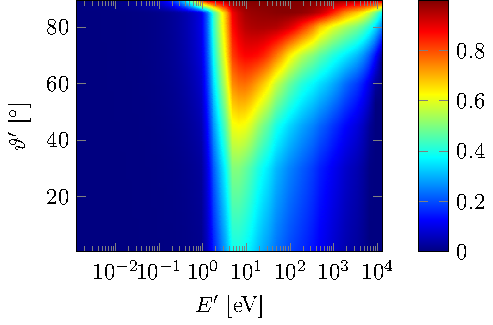
\includegraphics[width = 0.5\textwidth ]{Figures/RN.pdf}
	\caption{Particle reflection coefficient for deuterium projectiles on a carbon target.}
	\label{fig:RN}
\end{figure}

It is harder to calculate the other moment reflection coefficients (elaborating the integrals of Eqs.~\eqref{eq:Rmpar}, \eqref{eq:Rmperp}, \eqref{eq:Rp}, \eqref{eq:Rnn}, \eqref{eq:Rwwn}, and \eqref{eq:RE}) due to the specific format of the TRIM tables. Therefore, we use a Monte Carlo simulation with a very large amount of particles. For every combination of $v_{i}'$ and $\vartheta_{j}'$, we interpolate or extrapolate the whole TRIM table (e.g., Fig.~\ref{fig:trim}). Then, we launch a particle with speed $v_{i}'$, polar angle $\vartheta_{j}'$ and zero azimuthal angle and use the Monte Carlo procedure of Section~\ref{sec:MCbc}. This leads to a reflected speed $v_{k}$, polar angle $\vartheta_{k}$ and azimuthal angle $\varphi_{k}$. The process is repeated for $N$ particles. The moment reflection coefficient is estimated as
\begin{equation}
\hat{R}_{\mu}(v_{i}',\vartheta_{j}') = R_{\mathrm{N}}(v_{i}',\vartheta_{j}') \frac{1}{\mu(v_{i}',\vartheta_{j}',0)} \frac{1}{N} \sum_{k=1}^{N} \mu(v_{k},\vartheta_{k},\varphi_{k}),
\end{equation}
with the hat on top of $R$ indicating that it is a Monte Carlo estimation, and $\mu(v,\vartheta,\varphi)$ the particular moment, e.g., $\mu(v,\vartheta,\varphi) = v \sin \vartheta \cos \varphi$ for the parallel momentum reflection coefficient.

Fig.~\ref{fig:Rmoment} shows the results for deuterium impinging on carbon boundary material. For every combination of $v_{i}'$ and $\vartheta_{j}'$, $N = 10^{5}$ particles are used. Most moment reflection coefficients behave similarly as the particle reflection coefficient (Fig.~\ref{fig:RN}), with peak values for large incident angles and increase of the maximum value for fixed $\vartheta'$ when $\vartheta'$ increases. This is different for the density reflection coefficient (Fig.~\ref{fig:Rmp2}) due to the $1/v$ scaling in Eq.~\eqref{eq:Rnn}.
\begin{figure}[H]
	\centering
	\subfloat[Parallel momentum $\hat{R}_{\mathrm{m},||}$.]{
		\centering
		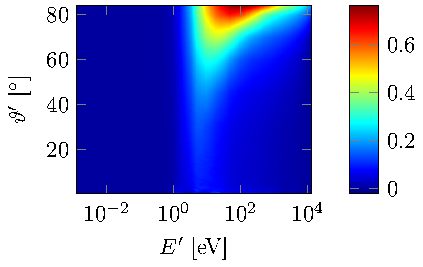
\includegraphics[width = 0.5\textwidth ]{Figures/Rmpar.pdf}
	}
	\subfloat[Perpendicular momentum $\hat{R}_{\mathrm{m},\perp}$.]{
		\centering
		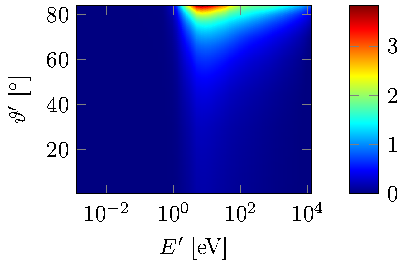
\includegraphics[width = 0.47\textwidth ]{Figures/Rmperp.pdf}
	} \\
	\subfloat[Pressure $\hat{R}_{p}$.]{
	\centering
	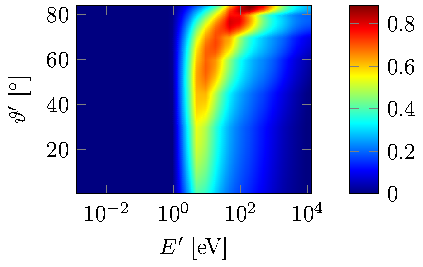
\includegraphics[width = 0.5\textwidth ]{Figures/Rmp1.pdf}
	}
	\subfloat[Density $\hat{R}_{\nn}$.]{
		\centering
		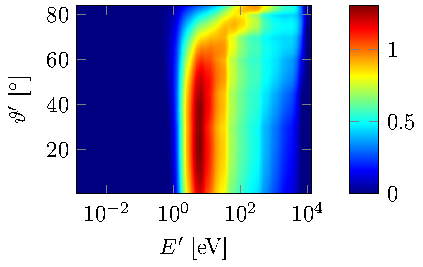
\includegraphics[width = 0.5\textwidth ]{Figures/Rmp2.pdf}
		\label{fig:Rmp2}
	} \\
	\subfloat[Toroidal velocity $\hat{R}_{\wwn}$.]{
	\centering
	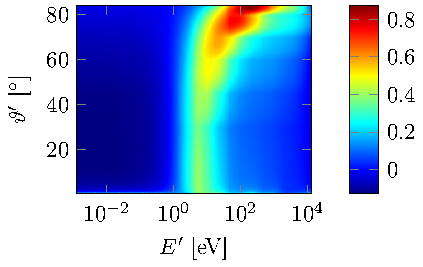
\includegraphics[width = 0.5\textwidth ]{Figures/Rmp3.pdf}
	}
	\subfloat[Energy $\hat{R}_{E}$.]{
		\centering
		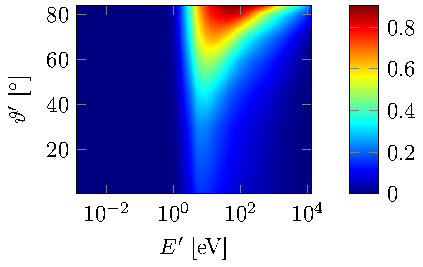
\includegraphics[width = 0.5\textwidth ]{Figures/RE.pdf}
	}
	\caption[TRIM moment reflection coefficients for deuterium projectiles on a carbon target.]{TRIM moment reflection coefficients for deuterium projectiles on a carbon target calculated with a Monte Carlo simulation.}
	\label{fig:Rmoment}
\end{figure}

\subsubsection{Resulting fluid boundary fluxes}
% ------------------------------------------------

We have characterized the TRIM database with seven moment reflection coefficients. Now, the integrals of Section~\ref{sec:boundaryfluxes} have to be calculated.

For the contributions of the incident neutrals (subscript $\nu-$), this can be done analytically. This leads to the following (particle, parallel momentum, and energy flux densities):
\begin{align}
\Gamma_{\nu-}^{\mathrm{n,diff}} =& - \frac{\nni\rcxm}{\nni\rcxm + \nne \rion} \left( \nn M^\mathrm{i}_{\nu} - \frac{1}{\nni\rcxm + \nne\rion} \left( \ddx{\nn}{\tau} M^\mathrm{i}_{\tau\nu} + \ddx{\nn}{\nu} M^\mathrm{i}_{\nu\nu} \right) \right), \label{eq:Gammanin2} \\
% -----------------------------------------------------------------------------------
\Gamma_{\mathrm{m},||,\nu-}^{\mathrm{n,diff}} =& -m \frac{\nni\rcxm}{\nni\rcxm + \nne\rion} \Bigg( \nn \left( \pit \left( \sin \alpha_{\nu} M^\mathrm{i}_{\tau\nu} + \cos \alpha_{\nu} M^\mathrm{i}_{\nu\nu} \right) + \pitt M^\mathrm{i}_{\phi\nu} \right) \nonumber \\
&- \frac{1}{\nni\rcxm + \nne\rion} \left( \ddx{\nn}{\tau} \left( \pit \left( \sin \alpha_{\nu} M^\mathrm{i}_{\tau\tau\nu} + \cos \alpha_{\nu} M^\mathrm{i}_{\tau\nu\nu} \right) + \pitt M^\mathrm{i}_{\phi\tau\nu} \right) \right. \nonumber \\
& \left. + \ddx{\nn}{\nu} \left( \pit \left( \sin \alpha_{\nu} M^\mathrm{i}_{\nu\nu\tau} + \cos \alpha_{\nu} \right) M^\mathrm{i}_{\nu\nu\nu} + \pitt M^\mathrm{i}_{\phi\nu\nu} \right) \right) \Bigg), \label{eq:Gammamompin} \\
% ----------------------------------------------------------------------------------
Q_{\nu-}^{\mathrm{n,diff}} =& -\frac{m}{2} \frac{\nni\rcxm}{\nni\rcxm + \nne\rion} \bigg ( \nn \left( M^\mathrm{i}_{\phi\phi\nu} + M^\mathrm{i}_{\tau\tau\nu} + M^\mathrm{i}_{\nu\nu\nu} \right) \nonumber \\
& - \frac{1}{\nni\rcxm + \nne \rion} \left( \ddx{\nn}{\tau} \left( M^\mathrm{i}_{\phi\phi\tau\nu} + M^\mathrm{i}_{\tau\tau\tau\nu} + M^\mathrm{i}_{\tau\nu\nu\nu} \right) \right. \nonumber \\
&\left. + \ddx{\nn}{\nu} \left( M^\mathrm{i}_{\phi\phi\nu\nu} + M^\mathrm{i}_{\tau\tau\nu\nu} + M^\mathrm{i}_{\nu\nu\nu\nu} \right) \right ) \bigg ), \label{eq:Qnin}
\end{align}
with
\begin{equation}
M^\mathrm{i}_{\alpha\beta\gamma\delta} = \int_{v_{\phi}'=-\infty}^{\infty} \int_{v_{\tau}'=-\infty}^{\infty} \int_{v_{\nu}' = - \infty}^{0} v_{\alpha}' v_{\beta}' v_{\gamma}' v_{\delta}' \widetilde{M}(v_{\phi}',v_{\tau}',v_{\nu}',\Vi,\Ti) \dd v_{\phi}' \dd v_{\tau}' \dd v_{\nu}',
\end{equation}

\noindent i.e., a certain moment of a Maxwellian distribution, with the subscripts indicating the particular velocity components by which the Maxwellian is multiplied. When using the drifting Maxwellian assumption instead of the diffusion assumption we get:

\begin{align}
\Gamma_{\nu-}^{\mathrm{n,Maxw}} =& - \nn M^\mathrm{n}_{\mathrm{n},\nu} ,   \label{eq:Gammanin2_maxw} \\
% -----------------------------------------------------------------------------------
\Gamma_{\mathrm{m},||,\nu-}^{\mathrm{n,Maxw}} =& -m \left( \nn \left( \pit \left( \sin \alpha_{\nu} M^\mathrm{n}_{\tau\nu} + \cos \alpha_{\nu} M^\mathrm{n}_{\nu\nu} \right) + \pitt M^\mathrm{n}_{\phi\nu} \right) \right), \label{eq:Gammamompin_maxw} \\
% ----------------------------------------------------------------------------------
Q_{\nu-}^{\mathrm{n,Maxw}} =& -\frac{m}{2} \left( \nn \left( M^\mathrm{n}_{\phi\phi\nu} + M^\mathrm{n}_{\tau\tau\nu} + M^\mathrm{n}_{\nu\nu\nu} \right) \right), \label{eq:Qnin_maxw}
\end{align}

with

\begin{equation}
M^\mathrm{n}_{\alpha\beta\gamma\delta} = \int_{v_{\phi}'=-\infty}^{\infty} \int_{v_{\tau}'=-\infty}^{\infty} \int_{v_{\nu}' = - \infty}^{0} v_{\alpha}' v_{\beta}' v_{\gamma}' v_{\delta}' \widetilde{M}(v_{\phi}',v_{\tau}',v_{\nu}',\Vn,\Tn) \dd v_{\phi}' \dd v_{\tau}' \dd v_{\nu}'\end{equation}

To obtain the fluid parallel momentum flux density of the incident neutrals $\Gamma_{\mathrm{m,f},||,\nu-}$, we have to subtract the pressure contribution from Eq.~\eqref{eq:Gammamompin}, as expressed by Eq.~\eqref{eq:Gammamompf}. Therefore, we also have to calculate the contributions from the incident neutrals to $\frac{m}{3} \int ||\vel||^{2} \frac{\Gamma^{\mathrm{n}}(\vel)}{|v_{\nu}|} \dd \vel$ (Eq.~\eqref{eq:v2fn}), $\nn'$ (Eq.~\eqref{eq:nnboundary}), and $\nn' \wwn'$ (Eq.~\eqref{eq:wwnboundary}). Elaborating these terms, gives for the diffusion approach
\begin{align}
\left [\frac{m}{3} \int ||\vel||^{2} \frac{\Gamma^{\mathrm{n}}(\vel)}{|v_{\nu}|} \dd \vel \right ]_{\nu-}^\mathrm{diff} =& \ \frac{m}{3} \frac{\nni\rcxm}{\nni\rcxm + \nne\rion} \bigg ( \nn \left( M_{\phi\phi}^\mathrm{i} + M_{\tau\tau}^\mathrm{i} + M_{\nu\nu}^\mathrm{i} \right) \nonumber \\
- & \frac{1}{\nni\rcxm + \nne\rion} \left( \ddx{\nn}{\tau} \left( M_{\phi\phi\tau}^\mathrm{i} + M_{\tau\tau\tau}^\mathrm{i} + M_{\nu\nu\tau}^\mathrm{i} \right) \right. \nonumber \\
+ & \left. \ddx{\nn}{\nu} \left( M_{\phi\phi\nu}^\mathrm{i} + M_{\tau\tau\nu}^\mathrm{i} + M_{\nu\nu\nu}^\mathrm{i} \right) \right) \bigg ), \label{eq:pnin} \\
% ------------------------------------------------------------------------------------------------
(n_{\mathrm{n},\nu-}')^\mathrm{diff} =& \ \frac{\nni\rcxm}{\nni\rcxm + \nne\rion} \bigg (\nn M^\mathrm{i} \nonumber \\
- & \frac{1}{\nni\rcxm + \nne\rion} \left (\ddx{\nn}{\tau} M^\mathrm{i}_{\tau} + \ddx{\nn}{\nu} M^\mathrm{i}_{\nu} \right ) \bigg ), \\
% ------------------------------------------------------------------------------------------------
\left [\nn'\wwn'\right ]_{\nu-}^\mathrm{diff} =& \ \frac{\nni\rcxm}{\nni\rcxm + \nne\rion} \bigg (\nn M_{\phi}^\mathrm{i} \nonumber \\
- & \frac{1}{\nni\rcxm + \nne\rion} \left (\ddx{\nn}{\tau} M_{\phi\tau}^\mathrm{i} + \ddx{\nn}{\nu} M_{\phi\nu}^\mathrm{i} \right ) \bigg ). \label{eq:wwnin}
\end{align}

For the drifting Maxwellian approach this becomes

\begin{align}
\left[ \frac{m}{3} \int ||\vel||^{2} \frac{\Gamma^{\mathrm{n}}(\vel)}{|v_{\nu}|} \dd \vel \right]_{\nu-}^\mathrm{Maxw} =& \ \frac{m}{3} \left( \nn \left( M_{\phi\phi}^\mathrm{n} + M_{\tau\tau}^\mathrm{n} + M_{\nu\nu}^\mathrm{n} \right) \right), \label{eq:pnin_maxw} \\
% ------------------------------------------------------------------------------------------------
(n_{\mathrm{n},\nu-}')^\mathrm{Maxw} =& \ \nn M^\mathrm{n}  \\
% ------------------------------------------------------------------------------------------------
\left [\nn'\wwn'\right ]_{\nu-}^\mathrm{Maxw} =& \ \nn M_{\phi}^\mathrm{n}. \label{eq:wwnin_maxw}
\end{align}

For the fast recycled and reflected contributions, the integrals can no longer be calculated analytically and they are evaluated numerically. To avoid the cost of recalculating the integrals every time the plasma state changes, the integrals are evaluated in advance for different values of the influencing plasma parameters. Every boundary flux density $\Gamma_{\mu}^{\mathrm{n}}$ of a particular moment $\mu$ can be written as
\begin{equation}
\Gamma_{\mu}^{\mathrm{n}} = \Gamma_{\mu,\nu-}^{\mathrm{n}} + \sum_{k}A_{\mu}^{k} \int_{v'=0}^{\infty} \int_{\vartheta'=0}^{\pi/2} \int_{\varphi'=0}^{2\pi} g_{\mu}^{k}(v',\vartheta',\varphi';{\bf R}) \fanorm(v',\vartheta',\varphi';\delta_{\mathrm{sh}}^{\mathrm{pot},k},\mathbf{V}_a,T_a) \dd v'\dd \vartheta' \dd \varphi', \label{eq:implementation}
\end{equation}
with $\Gamma_{\mu,\nu-}^{\mathrm{n}}$ the analytic expressions for the incident contributions (Eqs.~\eqref{eq:Gammanin2}-\eqref{eq:Qnin}, \eqref{eq:pnin}-\eqref{eq:wwnin}). The coefficient $A_{\mu}^{k}$ contains all terms that can be brought outside the integral (not functions of $v'$, $\vartheta'$, or $\varphi'$). The summation is used to distinguish between the different contributions. There is a contribution due to the recycled neutrals and three contributions of the reflected neutrals, respectively scaling with $\nn$, $\ddx{\nn}{\tau}$, and $\ddx{\nn}{\nu}$ (see Eq.~\eqref{eq:Gammanmin}). The integrand can be written as the product with a function $g_{\mu}^{k}(v',\vartheta',\varphi';{\bf R})$, which contains the needed TRIM reflection coefficients (present in ${\bf R}$). For the recycling contributions and the reflection contributions using the diffusion approximation, the Maxwellian distribution $\fanorm(v',\vartheta',\varphi';\delta_{\mathrm{sh}}^{\mathrm{pot},k},\mathbf{V}_a,T_a) \dd v'\dd \vartheta' \dd \varphi'$ is equal to the ion distribution $\finorm(v',\vartheta',\varphi';\delta_{\mathrm{sh}}^{\mathrm{pot},k},\Vi,\Ti)$ given by Eq.~\eqref{eq:finormdshpot}. The superscript $k$ for $\dshpot$ is needed to distinguish between the recycled and reflected neutrals. For the reflected neutrals using the diffusion approximation, $\delta_{\mathrm{sh}}^{\mathrm{pot},k} = 0$, whereas $\delta_{\mathrm{sh}}^{\mathrm{pot},k}$ is nonzero for the recycled neutrals if the boundary is not fully parallel to the magnetic field. For the reflected neutrals with the drifting Maxwellian assumption, $\fanorm(v',\vartheta',\varphi';\delta_{\mathrm{sh}}^{\mathrm{pot},k},\mathbf{V}_a,T_a) \dd v'\dd \vartheta' \dd \varphi'$ is equal to $\tilde{f}_\mathrm{n}(v',\vartheta',\varphi';0,\mathbf{V}_\mathrm{n},\Tn) \dd v'\dd \vartheta' \dd \varphi'$, given by Equation \eqref{eq:fnnorm}. Only the integral in Eq.~\eqref{eq:implementation} is calculated in advance and saved as a function of the sheath transmission coefficient, ion fluid velocity, and temperature:
\begin{equation}
\mathrm{RC}_{\mu}^{k}(\mathbf{V}_a,T_a) = \int_{v'=0}^{\infty} \int_{\vartheta'=0}^{\pi/2} \int_{\varphi'=0}^{2\pi} g_{\mu}^{k}(v',\vartheta',\varphi';{\bf R}) \fanorm(v',\vartheta',\varphi';\delta_{\mathrm{sh}}^{\mathrm{pot},k},\mathbf{V}_a,T_a) \dd v' \dd \vartheta' \dd \varphi'. \label{eq:Imu}
\end{equation}

To reduce the number of dependencies of $\mathrm{RC}_{\mu}^{k}$, we assume that $\mathbf{V}_a \approx \begin{bmatrix} u_{a,\phi} & 0 & 0 \end{bmatrix}^{T}$, expressed in the $(\phi,\tau,\nu)$ coordinate system. This assumption is valid for the ions if the pitch is sufficiently small such that the parallel direction almost coincides with the toroidal direction, and drifts are not included. For the neutrals in the drifting Maxwellian approximation, or for the ions when drifts are included, this assumption is less accurate. Even so, good fluid-kinetic agreement was achieved for cases with drifts in Ref. \cite{psi_wim}. Studying the role of the perpendicular bulk velocities, and finding a way to include them without making the databases unacceptably large, is subject of future work.  We evaluate Eq.~\eqref{eq:Imu} for 100 values of the Mach number $\mathcal{M}_{a,\phi} = u_{a,\phi}/\sqrt{2 T_a /m}$, uniformly distributed between 0 and 1.1 and 100 values for the temperature logarithmically distributed between 0.1 and 1\,000~eV. The midpoint integration rule is used with the discretized speed and polar angle from respectively Eq.~\eqref{eq:vdisc} and Eq.~\eqref{eq:thetadisc}, and the azimuthal angle $\varphi'$ discretized as
\begin{equation}
\varphi_{l}' = \frac{\pi}{400} + (l-1) \frac{\pi}{200}, \quad \text{for} \quad l = 1,\ldots, 400.
\end{equation}
Now, all integrated reflection coefficients are tabulated as a function of $\mathcal{M}_{a,\phi}$, $T_{a}$, and $\dshpot$.  During the simulation, we use linear interpolation for intermediate values of $\mathcal{M}_{a,\phi}$, $T_a$, and $\dshpot$.






